\documentclass[dvipdfmx]{beamer}
\usepackage{tutorial}
\title{計算機実験 --- 行列の対角化}

\begin{document}

\lstset{language={C},basicstyle=\ttfamily\scriptsize,showspaces=false,rulecolor=\color[cmyk]{0, 0.29,0.84,0}}

\begin{frame}
  \titlepage
  \tableofcontents
\end{frame}

\section{物理に現れる連立一次方程式}

\begin{frame}[t,fragile]{連立一次方程式の現れる例}
  \begin{itemize}
    \setlength{\itemsep}{1em}
  \item 微分方程式の初期値問題の陰解法
  \item 非線形連立方程式に対するニュートン法
    \[ {\bf x}' = {\bf x} - \Big( \frac{\partial {\bf f}({\bf x})}{\partial {\bf x}} \Big)^{-1} {\bf f}({\bf x}) \]
  \item 偏微分方程式の境界値問題の差分法による求解
  \item ベクトルに逆行列を掛ける代わりに連立一次方程式を解く場合が多い
    \[ {\bf x} = A^{-1} {\bf b} \ \ \Rightarrow \ \ A {\bf x} = {\bf b} \]
  \end{itemize}
\end{frame}

\begin{frame}[t,fragile]{ポアソン方程式の境界値問題}
  \begin{itemize}
    \setlength{\itemsep}{1em}
  \item 二次元ポアソン方程式
    \[ \frac{\partial^2 u(x,y)}{\partial x^2} + \frac{\partial^2 u(x,y)}{\partial y^2} = f(x,y) \qquad 0 \le x \le 1, \ 0 \le y \le 1\]
  \item ディリクレ型境界条件: $u(x,y) = g(x,y)$ on $\partial \Omega$
  \item 有限差分法により離散化
    \begin{itemize}
    \item $x$方向、$y$方向をそれぞれ$n$等分: $(x_i,y_j) = (i/n, j/n)$
    \item $(n+1)^2$個の格子点の上で$u(x_i,y_j)=u_{ij}$が定義される
    \item そのうち$4n$個の値は境界条件で定まる
    \item ポアソン方程式を中心差分で近似 ($h=1/n$)
      \[
      \frac{u_{i+1,j}-2u_{ij}+u_{i-1,j}}{h^2} + \frac{u_{i,j+1}-2u_{ij}+u_{i,j-1}}{h^2} = f_{ij}
      \]
      残り$(n-1)^2$個の未知数に対する連立一次方程式
    \end{itemize}
  \end{itemize}
\end{frame}

\begin{frame}[t,fragile]{ポアソン方程式の境界値問題}
  \begin{itemize}
    \setlength{\itemsep}{1em}
  \item ノイマン型境界条件の場合
    \begin{itemize}
    \item 境界上で$u(x,y)$の微分が定義される。
    \item 例) $\partial u(0,y) / \partial x = h(0,y)$
    \end{itemize}
  \item 境界条件を差分近似で表す
    \[
    \frac{u_{1j} - u_{0j}}{h} = h_{0j} \qquad j=1 \cdots (n-1)
    \]
    $(n+1)^2-4$個の未知数に対して、ポアソン方程式の差分近似とあわせて、合計$(n-1)^2+4(n-1)=(n+1)^2-4$個の連立一次方程式
  \end{itemize}
\end{frame}

% -*- coding: utf-8 -*-

\section{密行列の対角化}

\begin{frame}[t,fragile]{基本方針}
  \begin{itemize}
    %\setlength{\itemsep}{1em}
  \item やってはいけない方法: 特性方程式
    \[
    |\lambda E - A| = 0
    \]
    の係数を求めて、代数方程式として解く
    \begin{itemize}
    \item 数値的に不安定 (代数方程式の解は係数の誤差に対して敏感)
    \item 計算コスト大[$\sim O(N!)$]
    \end{itemize}
  \item スタンダードな方法: 行列を次々に直交変換して、対角行列(あるいは三重対角行列)に近づけていく
    \[
    A \rightarrow U_1^T A U_1 \rightarrow U_2^T (U_1^T A U_1) U_2 \rightarrow U_3^T (U_2^T (U_1^T A U_1) U_2) U_3 \rightarrow \cdots
    \]
  \item 固有値は変換された行列の固有値、固有ベクトルは変換後の行列の固有ベクトルに左から$U_1 U_2 U_3 \cdots$を掛けたもの
  \end{itemize}
\end{frame}

\begin{frame}[t,fragile]{Jacobi法}
  \begin{itemize}
    \setlength{\itemsep}{1em}
  \item 直交行列$U_{pq}$を以下のように選ぶ ($(p,p),(p,q),(q,p),(q,q)$成分を除くと単位行列)
    \[
    U_{pq} =
    \begin{bmatrix}
      1 \\
      & \ddots \\
      & & 1 \\
      & & & \cos \theta & & & \sin \theta \\
      & & & & 1 \\
      & & & & & 1 \\
      & & & -\sin \theta & & & \cos \theta \\
      & & & & & & & 1 \\
      & & & & & & & & \ddots \\
      & & & & & & & & & 1 \\
    \end{bmatrix}
    \]
  \end{itemize}
\end{frame}

\begin{frame}[t,fragile]{Jacobi法による相似変換}
  \begin{itemize}
    %\setlength{\itemsep}{1em}
  \item $B=U_{pq}^{-1} A U_{pq}$により、$A$の$p$行、$q$行、$p$列、$q$列のみが変更を受ける
    \begin{align*}
      b_{pk} &= b_{kp} = a_{pk} \cos \theta - a_{qk} \sin \theta \qquad k \ne p,q \\
      b_{qk} &= b_{kq} = a_{pk} \sin \theta + a_{qk} \cos \theta \qquad k \ne p,q \\
      b_{pp} &= \frac{a_{pp}+a_{qq}}{2} + \frac{a_{pp}-a_{qq}}{2} \cos 2 \theta - a_{pq} \sin 2 \theta \\
      b_{qq} &= \frac{a_{pp}+a_{qq}}{2} - \frac{a_{pp}-a_{qq}}{2} \cos 2 \theta + a_{pq} \sin 2 \theta \\
      b_{pq} &= b_{qp} = \frac{a_{pp}-a_{qq}}{2} \sin 2 \theta + a_{pq} \cos 2 \theta
    \end{align*}
  \item $b_{pq} = b_{qp} = 0$とするには、$\theta$を次のように選べば良い
    \[
    \tan 2 \theta = - \frac{2 a_{pq}}{a_{pp}-a_{qq}}
    \]
  \end{itemize}
\end{frame}

\begin{frame}[t,fragile]{Jacobi法の収束}
  \begin{itemize}
    %\setlength{\itemsep}{1em}
  \item 相似変換により対角和は不変に保たれるので
    \[
      {\rm tr} \, A^T A = {\rm tr} \, B^T B \ \ \Rightarrow \ \
      \sum_{i,j} a_{ij}^2 = \sum_{i,j} b_{ij}^2
    \]
  \item 一方、この変換で
    \[
    b_{pp}^2 + b_{qq}^2 = b_{pp}^2 + 2 b_{pq}^2 + b_{qq}^2 = a_{pp}^2 + 2 a_{pq}^2 + a_{qq}^2
    \]
    すなわち、変換により、対角成分の二乗和は増加する $\Rightarrow$ 非対角成分の二乗和は単調減少
  \item 全ての非対角成分が十分小さくなるまで繰り返す
  \item 固有値=対角成分、固有ベクトル$=U_1 U_2 U_3 \cdots$
  \end{itemize}
\end{frame}

\begin{frame}[t,fragile]{3重対角化}
  \begin{itemize}
    %\setlength{\itemsep}{1em}
  \item 対角化は有限回の手続きでは行えない
  \item 3重対角化であれば、$O(n^3)$の有限回の計算で決定論的に行える
  \item Givens変換: Jacobi変換と同じ相似変換を利用
    \begin{itemize}
    \item $U_{32}$で(3,1)と(1,3)を消去 $\Rightarrow$ $U_{42}$で(4,1)と(1,4)を消去 $\Rightarrow$ $U_{52}$で(5,1)と(1,5)を消去 $\Rightarrow$ $U_{62},\cdots,U_{n,2}$ $\Rightarrow$ $U_{43},U_{53},\cdots,U_{n,3}$ $\Rightarrow$ $\cdots$ $\Rightarrow$ $U_{n,n-1}$で($n,n-2$)と($n-2,n$)を消去
    \item $(4/3)n^3$回の乗算と$(2/3)n^3$回の加減算で3重対角化される
    \end{itemize}
  \item Householder変換: $U = E - 2 w w^T / |w|^2$
    \begin{itemize}
    \item $(2/3)n^3$回の乗算と加減算で3重対角化される
    \item Givens変換に比べ少し効率的なので、こちらが広く使われている
    \end{itemize}
  \end{itemize}
\end{frame}

\begin{frame}[t,fragile]{3重対角行列の対角化}
  \begin{itemize}
    %\setlength{\itemsep}{1em}
  \item 二分法、QR分解、分割統治法、MRRRなど様々な方法が知られている
  \item 固有ベクトル
    \begin{itemize}
    \item QR分解では3重対角行列の固有ベクトルも同時に求まる
    \item あるいは、固有値を求めた後、逆反復法を用いて固有ベクトルを求める
    \end{itemize}
  \item 逆反復法
    \begin{itemize}
    \item 近似固有値を$\mu$とするとき、行列$(A - \mu E)^{-1}$を考えると、固有ベクトルは$A$と同じ、固有値は$(\lambda-\mu)^{-1}$。
    \item $\mu$が十分に正確であれば、$(\lambda-\mu)^{-1}$は絶対値最大の固有値。行列$(A - \mu E)^{-1}$を適当な初期ベクトルにかけ続けると$\lambda$に対応する固有ベクトルに収束(c.f. べき乗法)
    \item 実際には$(A-\mu E) x' = x$という連立方程式を繰り返し解く
    \end{itemize}
  \end{itemize}
\end{frame}

\begin{frame}[t,fragile]{LAPACKの対角化ルーチン}
  \begin{itemize}
    %\setlength{\itemsep}{1em}
  \item 様々な対角化ルーチンが準備されている
    \begin{itemize}
    \item 倍精度実対称行列の対角化 {\tt dsyev}
      \url{http://www.netlib.org/lapack/explore-html/dd/d4c/dsyev_8f.html}
    \item Fortranによる関数宣言
\begin{lstlisting}
subroutine dsyev(character JOBZ, character UPLO,
  integer N, double precision, dimension(lda, *) A,
  integer LDA, double precision, dimension(*) W,
  double precision, dimension(*) WORK,
  integer LWORK, integer INFO)		
\end{lstlisting}
    \end{itemize}
  \item 他にも{\tt dsyevd}、{\tt dsyevr}、{\tt dsyevx}などがある \\
    3重対角化までは同じ。3重対角行列の対角化が異なる
  \item 単精度版の{\tt ssyev}、複素(エルミート行列)版の{\tt zheev}など
  \item {\tt dsyev}の使用例: \href{https://github.com/todo-group/computer-experiments/blob/master/exercise/eigenvalue_problem/diag.c}{diag.c}
  \end{itemize}
\end{frame}

\begin{frame}[t,fragile]{複素エルミート行列の固有分解}
  \begin{itemize}
    %\setlength{\itemsep}{1em}
  \item 固有値は実数
  \item これまでの方法がそのまま使える (ただし、転置 $\rightarrow$ 複素転置)
  \item 実対称行列用のサブルーチンを使っての対角化も可能
    \begin{itemize}
    \item エルミート行列を実部と虚部に分ける: $A = R + iW$
    \item エルミート行列の固有値問題 $(R + iW)(u+iv) = \lambda(u+iv)$を$2N \times 2N$の実対称行列の問題に書き換える
      \[
      \begin{pmatrix} R & -W \\ W & R \end{pmatrix}
      \begin{pmatrix} u \\ v \end{pmatrix}
      = 
      \lambda \begin{pmatrix} u \\ v \end{pmatrix}
      \]
    \item 固有値は同じ固有値が2度づつ現れる
    \item 対応する複素行列の固有ベクトルは、$u+iv$と$-v+iu$
    \end{itemize}
  \end{itemize}
\end{frame}

\begin{frame}[t,fragile]{QR法}
  \begin{itemize}
    %\setlength{\itemsep}{1em}
  \item QR分解
    \begin{itemize}
    \item 行列$A$を直交(エルミート)行列$Q$と上三角行列$R$の積に分解: $A=QR$
    \item Gram-Schmidtの直交化と等価
    \end{itemize}
  \item QR法による固有値と固有ベクトルの計算
    \begin{itemize}
    \item 行列$A_1$をQR分解($A_1=Q_1R_1$) → $A_2 = R_1Q_1$ 
    \item 行列$A_2$をQR分解($A_2=Q_2R_2$) → $A_3 = R_2Q_2$ 
    \item 行列$A_k$をQR分解($A_k=Q_kR_k$) → $A_{k+1} = R_kQ_k$
    \item 繰り返していくと対角より下の全ての成分は零に収束し、対角成分は固有値に収束する(証明略)
    \end{itemize}
  \item 連続した直交変換: $A_{k+1} = R_kQ_k = Q_k^{-1}Q_kR_kQ_k = Q_k^{-1}A_kQ_k$
    \begin{itemize}
    \item $A_1$が対称(エルミート)三重対角行列の場合、$A_k$も対称(エルミート)三重対角
    \item 密行列に対して最初からQR法を適用するより、Householder法で三重対角化した後で使う方が効率がよい
    \end{itemize}
  \end{itemize}
\end{frame}


% -*- coding: utf-8 -*-

\documentclass[10pt,dvipdfmx]{beamer}
\usepackage{tutorial}

\begin{document}
\section{ビット表現}
%-*- coding:utf-8 -*-

\begin{frame}[t,fragile]{ビット表現}
  \begin{itemize}
    %\setlength{\itemsep}{1em}
  \item スピン状態($\uparrow$ / $\downarrow$)や量子ビット状態($|0\rangle$ / $|1\rangle$を表現するには二進数を考えるのが便利
    \begin{itemize}
    \item スピン数(量子ビット数): $N$
    \item 状態数: $2^N$
    \item 整数を二進数表現したときの下から$i$番目($i=0,1,\ldots,N-1$)の数字(0 / 1)を$i$番目のスピン状態($\uparrow$ / $\downarrow$)あるいは$i$番目の量子ビット状態($|0\rangle$ / $|1\rangle$)に対応させる
    \end{itemize}
  \item $N=3$の例
    \begin{itemize}
    \item $0 \rightarrow 000$: $\uparrow\uparrow\uparrow$ \ $|000\rangle$
    \item $1 \rightarrow 001$: $\uparrow\uparrow\downarrow$ \ $|001\rangle$
    \item $2 \rightarrow 010$: $\uparrow\downarrow\uparrow$ \ $|010\rangle$
    \item $3 \rightarrow 011$: $\uparrow\downarrow\downarrow$ \ $|011\rangle$
    \item $4 \rightarrow 100$: $\downarrow\uparrow\uparrow$ \ $|100\rangle$
    \item $5 \rightarrow 101$: $\downarrow\uparrow\downarrow$ \ $|101\rangle$
    \item $6 \rightarrow 110$: $\downarrow\downarrow\uparrow$ \ $|110\rangle$
    \item $7 \rightarrow 111$: $\downarrow\downarrow\downarrow$ \ $|111\rangle$
    \end{itemize}
  \end{itemize}
\end{frame}

%-*- coding:utf-8 -*-

\begin{frame}[t,fragile]{ビット表現}
  \begin{itemize}
    %\setlength{\itemsep}{1em}
  \item 特定のビットの取り出し
    \begin{itemize}
    \item シフト演算(\verb+>>+)とAND演算(\verb+&+)を利用 \ 例)

      3番目($i=3$)のビット(0 / 1)を取り出す: \verb+(s>>3)&1+

      3番目($i=3$)のスピン状態($\sigma_3 = \pm 1$)を取り出す: \verb+1-2*((s>>3)&1)+

      $\sigma_i \sigma_j$の計算: \verb+(1-2*((s>>i)&1)) * (1-2*((s>>j)&1))+

    \item {\color{red} $i$は0から数える}ことに注意($i=0,1,\ldots,N-1$)
    \item ビットAND (\verb+&+)と論理AND (\verb+&&+)との違いに注意
    \end{itemize}
  \item 特定のビットのフリップ(反転)
    \begin{itemize}
    \item シフト演算(\verb+<<+)とXOR(排他的論理和)演算(\verb+^+)を利用 \ 例)
      
      3番目($i=3$)のビットを反転: \verb+s^(1<<3)+
    \end{itemize}
  \item $N$ビット全てが1の状態を作る
    \begin{itemize}
    \item \verb+(1<<N)-1+
    \end{itemize}
  \item $N$重のforループを書く代わりに、状態を1つの$N$ビットの整数($s=0,\cdots,2^N-1$)で表し、ひとつのループに
  \end{itemize}
\end{frame}

\section{疎行列の扱い}
\begin{frame}[t,fragile]{疎行列}
  \begin{itemize}
    \setlength{\itemsep}{1em}
  \item 疎行列: 非零の要素の数が非常に少ない行列
    \begin{itemize}
    \item 全ての要素($N^2$)を保存しておくのはメモリの無駄
    \item 行列ベクトル積の計算量(通常$O(N^2)$)も削減の余地あり
    \end{itemize}
  \item 疎行列の格納
    \begin{itemize}
    \item 三重対角行列(一次元ラプラシアンなど): 例) \href{https://github.com/todo-group/computer-experiments/blob/master/exercise/eigenvalue_problem/tridiagonal.c}{\texttt{tridiagonal.c}}

      対角成分+副対角成分を3本のベクトルに保存しておけばよい

      対称(エルミート)行列の場合は副対角はどちらか1本だけでよい

      LAPACKの三重対角行列用のソルバー(\href{https://netlib.org/lapack/explore-html/dc/dd2/group__double_o_t_h_e_reigen_gaaa6df51cfd92c4ab08d41a54bf05c3ab.html}{\texttt{DSTEV}}, \href{https://netlib.org/lapack/explore-html/d1/d40/group__double_g_tcomputational_ga8ca64e542924cec56cbe9837b77d25b7.html}{\texttt{DGTTRF}}など)にはこの形式の行列を渡す

    \item 一般の疎行列: 例) \href{https://github.com/todo-group/computer-experiments/blob/master/exercise/eigenvalue_problem/sparse.c}{\texttt{sparse.c}}

      各行で非零の要素の場所(列)とその値をベクトルに保存する

      CRS (Compressed Row Storage)形式とも呼ばれる

    \item matfree形式: 例) \href{https://github.com/todo-group/computer-experiments/blob/master/exercise/eigenvalue_problem/matfree.c}{\texttt{matfree.c}}

      要素は保存せず、その場で非零の場所と要素を計算する

      FTCS法を行列形式を使わずに素直に実装するのと同じ

      横磁場イジング模型のハミルトニアンの掛け算などでも使える
    \end{itemize}
  \end{itemize}
\end{frame}

\end{document}

\section{特異値分解}

\begin{frame}[t,fragile]{一般の非正方行列の場合}
  \begin{itemize}
    %\setlength{\itemsep}{1em}
  \item 特異値分解(SVD: Singular Value Decomposition)
  \item 任意の$m \times n$実行列$A$は
    \[
    A = U \Lambda V^T
    \]
    の形に(一意に)分解できる ($k=\min(m,n)$)
  \item $U$: $(m \times k)$行列(列ベクトルは互いに正規直交) \\
    $V$: $(n \times k)$行列(列ベクトルは互いに正規直交) \\
    $\Lambda = \text{diag}(\lambda_1,\lambda_2,\cdots,\lambda_k)$ \ \ ($\lambda_1\ge\lambda_2\ge\cdots\ge\lambda_k\ge 0$) 特異値
  \item ベクトル表示 (行列をランク1の行列で分解)
    \[
    A = \sum_{i=1}^k \lambda_i u_i v_i^{T}
    \]
  \end{itemize}
\end{frame}

\begin{frame}[t,fragile]{特異値分解の例}
  \[
  \begin{split}
    \begin{pmatrix}
      1 & 2 & 3 \\
      6 & 4 & 5 \\
      8 & 9 & 7 \\
      10 & 11 & 12
    \end{pmatrix} =&
    \begin{pmatrix}
      -0.14 & -0.62 & -0.05 \\
      -0.34 & \ \ \,0.37 & \ \ \,0.81 \\
      -0.55 & \ \ \,0.54 & -0.58 \\
      -0.75 & -0.44 & \ \ \,0.06      
    \end{pmatrix} \\
    &\times
    \begin{pmatrix}
      25.35 & 0 & 0 \\
      0 & 2.15 & 0 \\
      0 & 0 & 1.71
    \end{pmatrix}
    \begin{pmatrix}
      -0.56 & -0.59 & -0.59 \\
      \ \ \,0.68 & \ \ \,0.09 & -0.73 \\
      \ \ \,0.48 & -0.81 & \ \ \,0.35
    \end{pmatrix}
  \end{split}
  \]
\end{frame}

\begin{frame}[t,fragile]{完全特異値分解 (full SVD)}
  \[
  \begin{split}
    \begin{pmatrix}
      1 & 2 & 3 \\
      6 & 4 & 5 \\
      8 & 9 & 7 \\
      10 & 11 & 12
    \end{pmatrix} =&
    \begin{pmatrix}
      -0.14 & -0.62 & -0.05 & {\color{red} -0.77} \\
      -0.34 & \ \ \,0.37 & \ \ \,0.81 & {\color{red} -0.29} \\
      -0.55 & \ \ \,0.54 & -0.58 & {\color{red} -0.29} \\
      -0.75 & -0.44 & \ \ \,0.06 & {\color{red} \ \ \,0.48}
    \end{pmatrix} \\
    &\times
    \begin{pmatrix}
      25.35 & 0 & 0 \\
      0 & 2.15 & 0 \\
      0 & 0 & 1.71 \\
      {\color{red} 0} & {\color{red} 0} & {\color{red} 0}
    \end{pmatrix}
    \begin{pmatrix}
      -0.56 & -0.59 & -0.59 \\
      \ \ \,0.68 & \ \ \,0.09 & -0.73 \\
      \ \ \,0.48 & -0.81 & \ \ \,0.35
    \end{pmatrix}
  \end{split}
  \]
  \begin{itemize}
    % \setlength{\itemsep}{1em}
  \item $U$, $V$が直交行列になるように、足りない基底ベクトルを追加
  \item こちらを「SVD」、もともとの分解を「thin SVD」と呼ぶこともある
  \end{itemize}
\end{frame}

\begin{frame}[t,fragile]{LAPACKによる特異値分解}
  \begin{itemize}
    %\setlength{\itemsep}{1em}
  \item 倍精度実行列の特異値分解 {\tt dgesvd}
    \url{http://www.netlib.org/lapack/explore-html/d8/d2d/dgesvd_8f.html}
  \item Fortranによる関数宣言
\begin{lstlisting}
subroutine dgesvd(character JOBU, character JOBVT,
  integer M, integer N,
  double precision, dimension(lda, *) A,
  integer LDA, double precision, dimension(*) S,
  double precision, dimension(ldu, *) U, integer LDU,
  double precision, dimension(ldvt, *) VT,
  integer LDVT,
  double precision, dimension(*) WORK, integer LWORK,
  integer INFO)
\end{lstlisting}
  \item {\tt dgesvd}の使用例: \href{https://github.com/todo-group/computer-experiments/blob/master/exercise/svd/svd.c}{svd.c} (SVD), \href{https://github.com/todo-group/computer-experiments/blob/master/exercise/svd/full_svd.c}{full\_svd.c} (完全SVD)
    \begin{itemize}
    \item コンパイル方法: {\tt cc -o svd svd.c -llapack -lblas -lm}
    \item 実行方法: {\tt ./svd matrix2.dat}
    \end{itemize}
  \end{itemize}
\end{frame}

\begin{frame}[t,fragile]{固有値分解との関係}
  \begin{itemize}
    %\setlength{\itemsep}{1em}
  \item 半正定値実対称行列の場合

    「固有値分解」と「特異値分解」は等価
  \item 一般の(非正方)実行列$A$の場合
    \begin{itemize}
      %\setlength{\itemsep}{1em}
    \item 完全SVD  $A=U \Lambda V^T$を考えると
    \item $B=A^T A = V \Lambda U^T U \Lambda V^T = V \Lambda^2 V^T$は実対称行列

      固有値:$\lambda_i^2$、固有ベクトル$V$
    \item $C=A A^T = U \Lambda V^T V \Lambda U^T = U \Lambda^2 U^T$も実対称行列

      固有値:$\lambda_i^2$、固有ベクトル$U$
    \end{itemize}
  \end{itemize}
\end{frame}

\begin{frame}[t,fragile]{特異値分解が役に立つ例}
  \begin{itemize}
    %\setlength{\itemsep}{1em}
  \item 連立一次方程式の最小二乗解
  \item 行列の低ランク近似
  \item 画像圧縮
  \end{itemize}
\end{frame}

\begin{frame}[t,fragile]{特異な(特異に近い)連立一次方程式}
  \begin{itemize}
    %\setlength{\itemsep}{1em}
  \item ランク$r$の$m \times n$行列$A$のfull SVDを考える
    \[
    A = \begin{pmatrix} U_1 U_2 \end{pmatrix} \begin{pmatrix} \Lambda_1 & 0 \\ 0 & 0 \end{pmatrix} \begin{pmatrix} V_1 V_2 \end{pmatrix}^T = U_1 \Lambda_1 V_1^T
    \]
    $U_1$: $m \times r$, $U_2$: $m \times (m-r)$, $\Lambda_1$: $r \times r$, $V_1$: $n \times r$, $V_2$: $n \times (n-r)$
  \item $r \ne n$のとき、方程式$Ax=b$は無限個の解をもつ、あるいは解なし
  \item 無限個の解をもつ場合($U_1U_1^Tb=b$)の一般解
    \[
    x = V_1 \Lambda_1^{-1} U_1^T b + V_2 z
    \]
    $z$は$(n-r)$次元の任意のベクトル
  \end{itemize}
\end{frame}

\begin{frame}[t,fragile]{一般化逆行列と最小二乗解}
  \begin{itemize}
    %\setlength{\itemsep}{1em}
  \item $V_1$と$V_2$の列ベクトルは全て直交する。一般解のうちノルム$|x|^2$が最小となるのは$z=0$のとき
    \[
    x = A^\dagger b \ \ \ \ A^\dagger = V \begin{pmatrix} \Lambda^{-1} & 0 \\ 0 & 0 \end{pmatrix} U^T
    \]
  \item $A^\dagger$: Moore-Penroseの一般化逆行列 (1/0を0とおくことに相当)
  \item $Ax=b$が解を持たない場合にも最良解を与える
  \item 零に非常に近い特異値がある場合も、それらを零とみなすことで数値的に安定した解がえられる
  \end{itemize}
\end{frame}

\begin{frame}[t,fragile]{行列の低ランク近似}
  \begin{itemize}
    %\setlength{\itemsep}{1em}
  \item ランク$r$ ($r<k$)の行列のうち、行列$A$を「最も良く近似」する$\tilde{A}$を選ぶ
  \item 「最も良く近似」= フロベニウスノルム$||A-\tilde{A}||_\mathrm{F}$を最小化
    \[
    ||X||^2_\mathrm{F} \equiv \sum_{ij} x_{ij}^2
    \]
  \item 特異値のうち大きなものから$r$個とり、残りを零とした
    \[
    \tilde{\Lambda} = \text{diag}(\lambda_1,\cdots,\lambda_r,0,\cdots,0)
    \]
    を使い
    \[
    \tilde{A} = U \tilde{\Lambda} V^T
    \]
    を作れば良い (Eckart-Youngの定理)
  \end{itemize}
\end{frame}

\begin{frame}[t,fragile]{行列の低ランク近似の例}
  \[
  \begin{split}
    &\begin{pmatrix}
      -0.14 & -0.62 & -0.05 \\
      -0.34 & \ \ \,0.37 & \ \ \,0.81 \\
      -0.55 & \ \ \,0.54 & -0.58 \\
      -0.75 & -0.44 & \ \ \,0.06      
    \end{pmatrix}
    \begin{pmatrix}
      25.35 & 0 & 0 \\
      0 & 2.15 & 0 \\
      0 & 0 & 0
    \end{pmatrix} \\
    & \times
    \begin{pmatrix}
      -0.56 & -0.59 & -0.59 \\
      \ \ \,0.68 & \ \ \,0.09 & -0.73 \\
      \ \ \,0.48 & -0.81 & \ \ \,0.35
    \end{pmatrix}
    = 
    \begin{pmatrix}
      1.04 & 1.93 & 3.03 \\
      5.33 & 5.12 & 4.52 \\
      8.47 & 8.21 & 7.34 \\
      9.95 & 11.1 & 12.0 \\
    \end{pmatrix}
  \end{split}
  \]
  \begin{itemize}
    % \setlength{\itemsep}{1em}
  \item それなりに悪くない近似が得られる
  \item 誤差(フロベニウスノルム) = 1.71 (無視した特異値の二乗和の平方根)
  \end{itemize}
\end{frame}

\begin{frame}[t,fragile]{Eckart-Youngの定理の証明}
  \begin{itemize}
    %\setlength{\itemsep}{1em}
  %\item $A=U \Lambda V^T$のように(完全)SVDされているとする
  \item $A$を近似する行列$X$ (ランク$\le r$)を考えると
    \[
    ||A-X||_\mathrm{F}^2 = \sum_{ij}(a_{ij}-x_{ij})^2 = \text{tr} [(A-X)(A-X)^T]
    \]
    を最小化すればよい。完全SVDについて$UU^T=E_m$, $VV^T = E_n$より
    \[
    \begin{split}
      ||A-X||_\mathrm{F}^2 &= \text{tr} [UU^T(A-X)VV^T(A-X)^T] \\
      %% &= \text{tr} [U^T(A-X)V (U^T(A-X)V)^T] \\
      &= \text{tr} [(\Lambda-G)(\Lambda-G)^T]  \ \ \ (G \equiv U^TXV)\\
      &= \sum_i^k (\lambda_i - g_{ii})^2 + \sum_i \sum_{j \ne i} g_{ij}^2
    \end{split}
    \]
    ランク$r$以下で、$||A-X||_\mathrm{F}^2$を最小化するには、$g_{ii}=\lambda_i$ ($i=1 \cdots r$)、それ以外は全て零とすればよい
  \end{itemize}
\end{frame}

\begin{frame}[t,fragile]{特異値分解による画像圧縮}
  \begin{itemize}
  \item 特異値の分布とランク$r$近似 ($1614 \times 2178$グレイスケール写真)
    
    \hspace*{-3em}\resizebox{0.27\textwidth}{!}{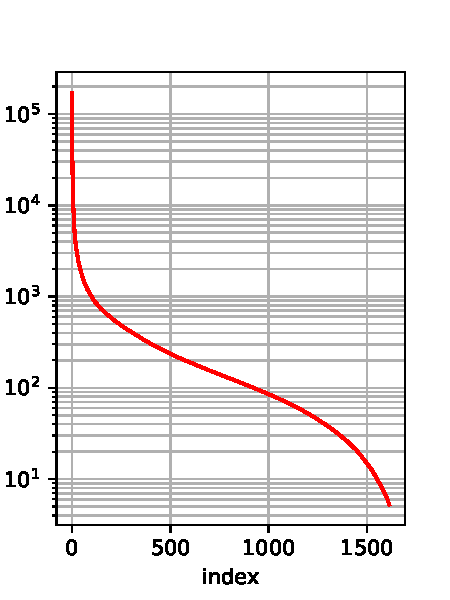
\includegraphics{image/singular_values.pdf}}

    \vspace*{-11em}\hfill
    \begin{tabular}{cccc}
      $r=1$ & $r=2$ & $r=3$ & $r=4$ \\
      \resizebox{0.15\textwidth}{!}{
\includegraphics{image/gray_picture_r1.pdf}} &
      \resizebox{0.15\textwidth}{!}{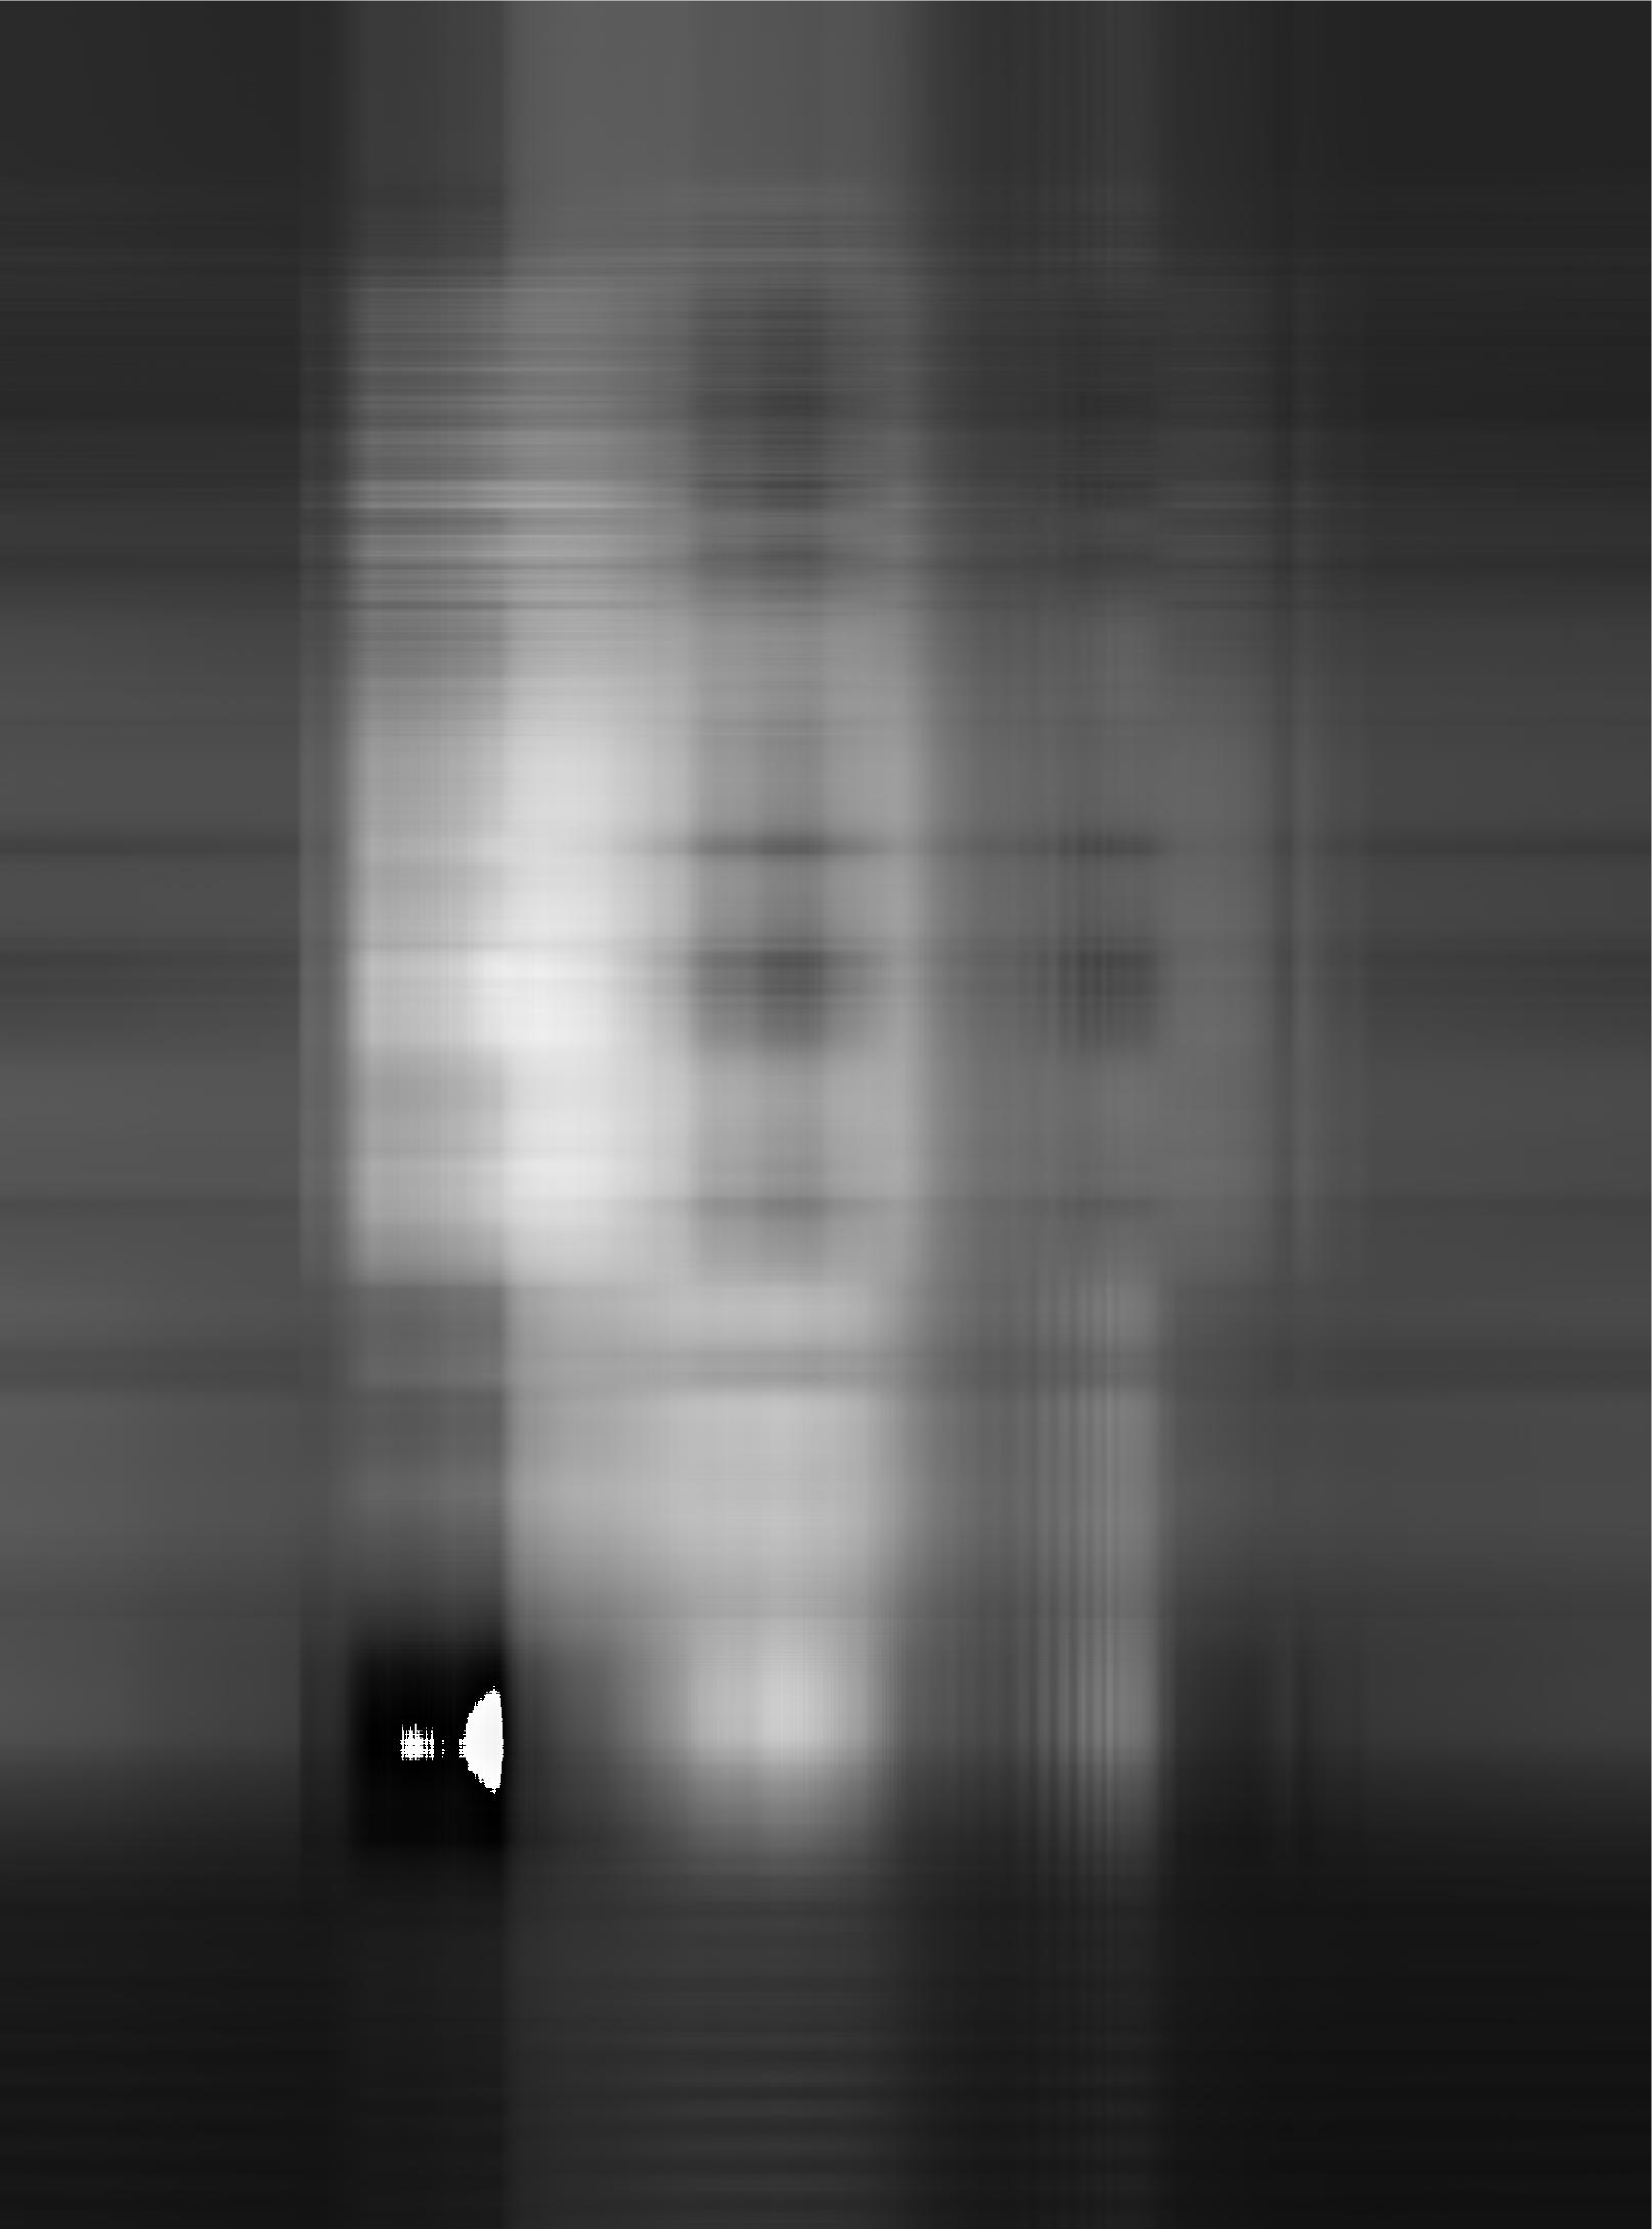
\includegraphics{image/gray_picture_r2.pdf}} &
      \resizebox{0.15\textwidth}{!}{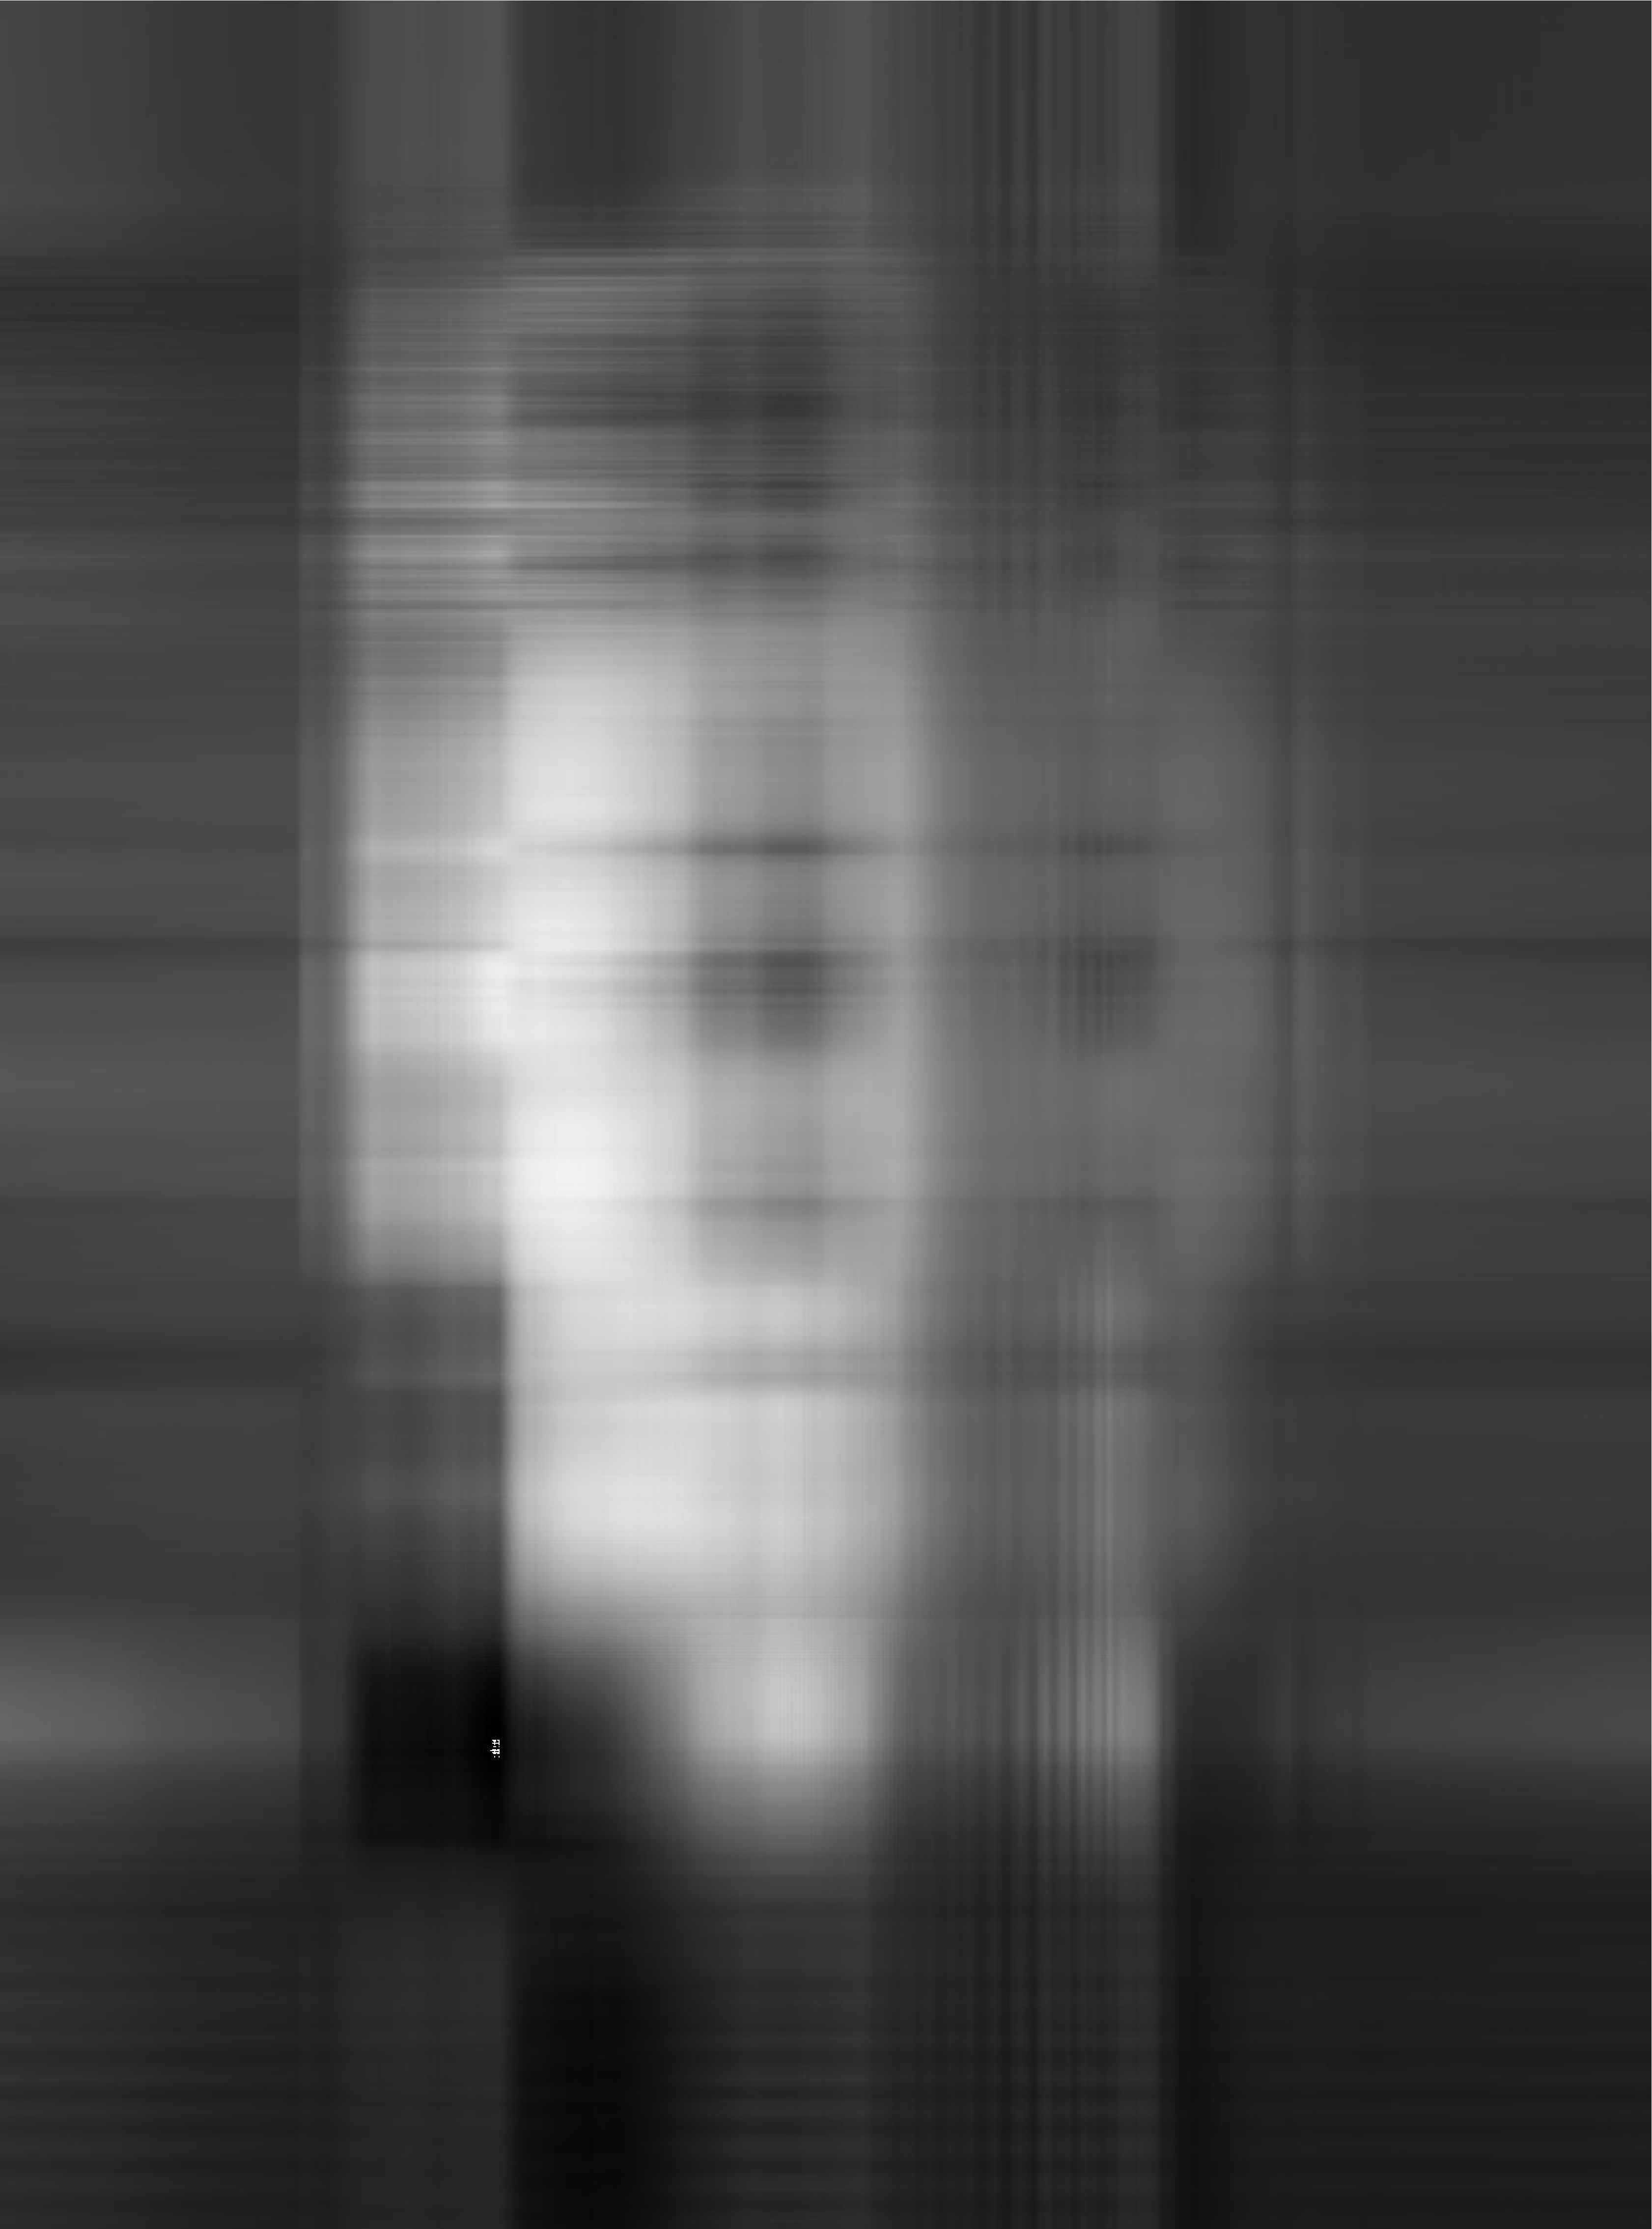
\includegraphics{image/gray_picture_r3.pdf}} &
      \resizebox{0.15\textwidth}{!}{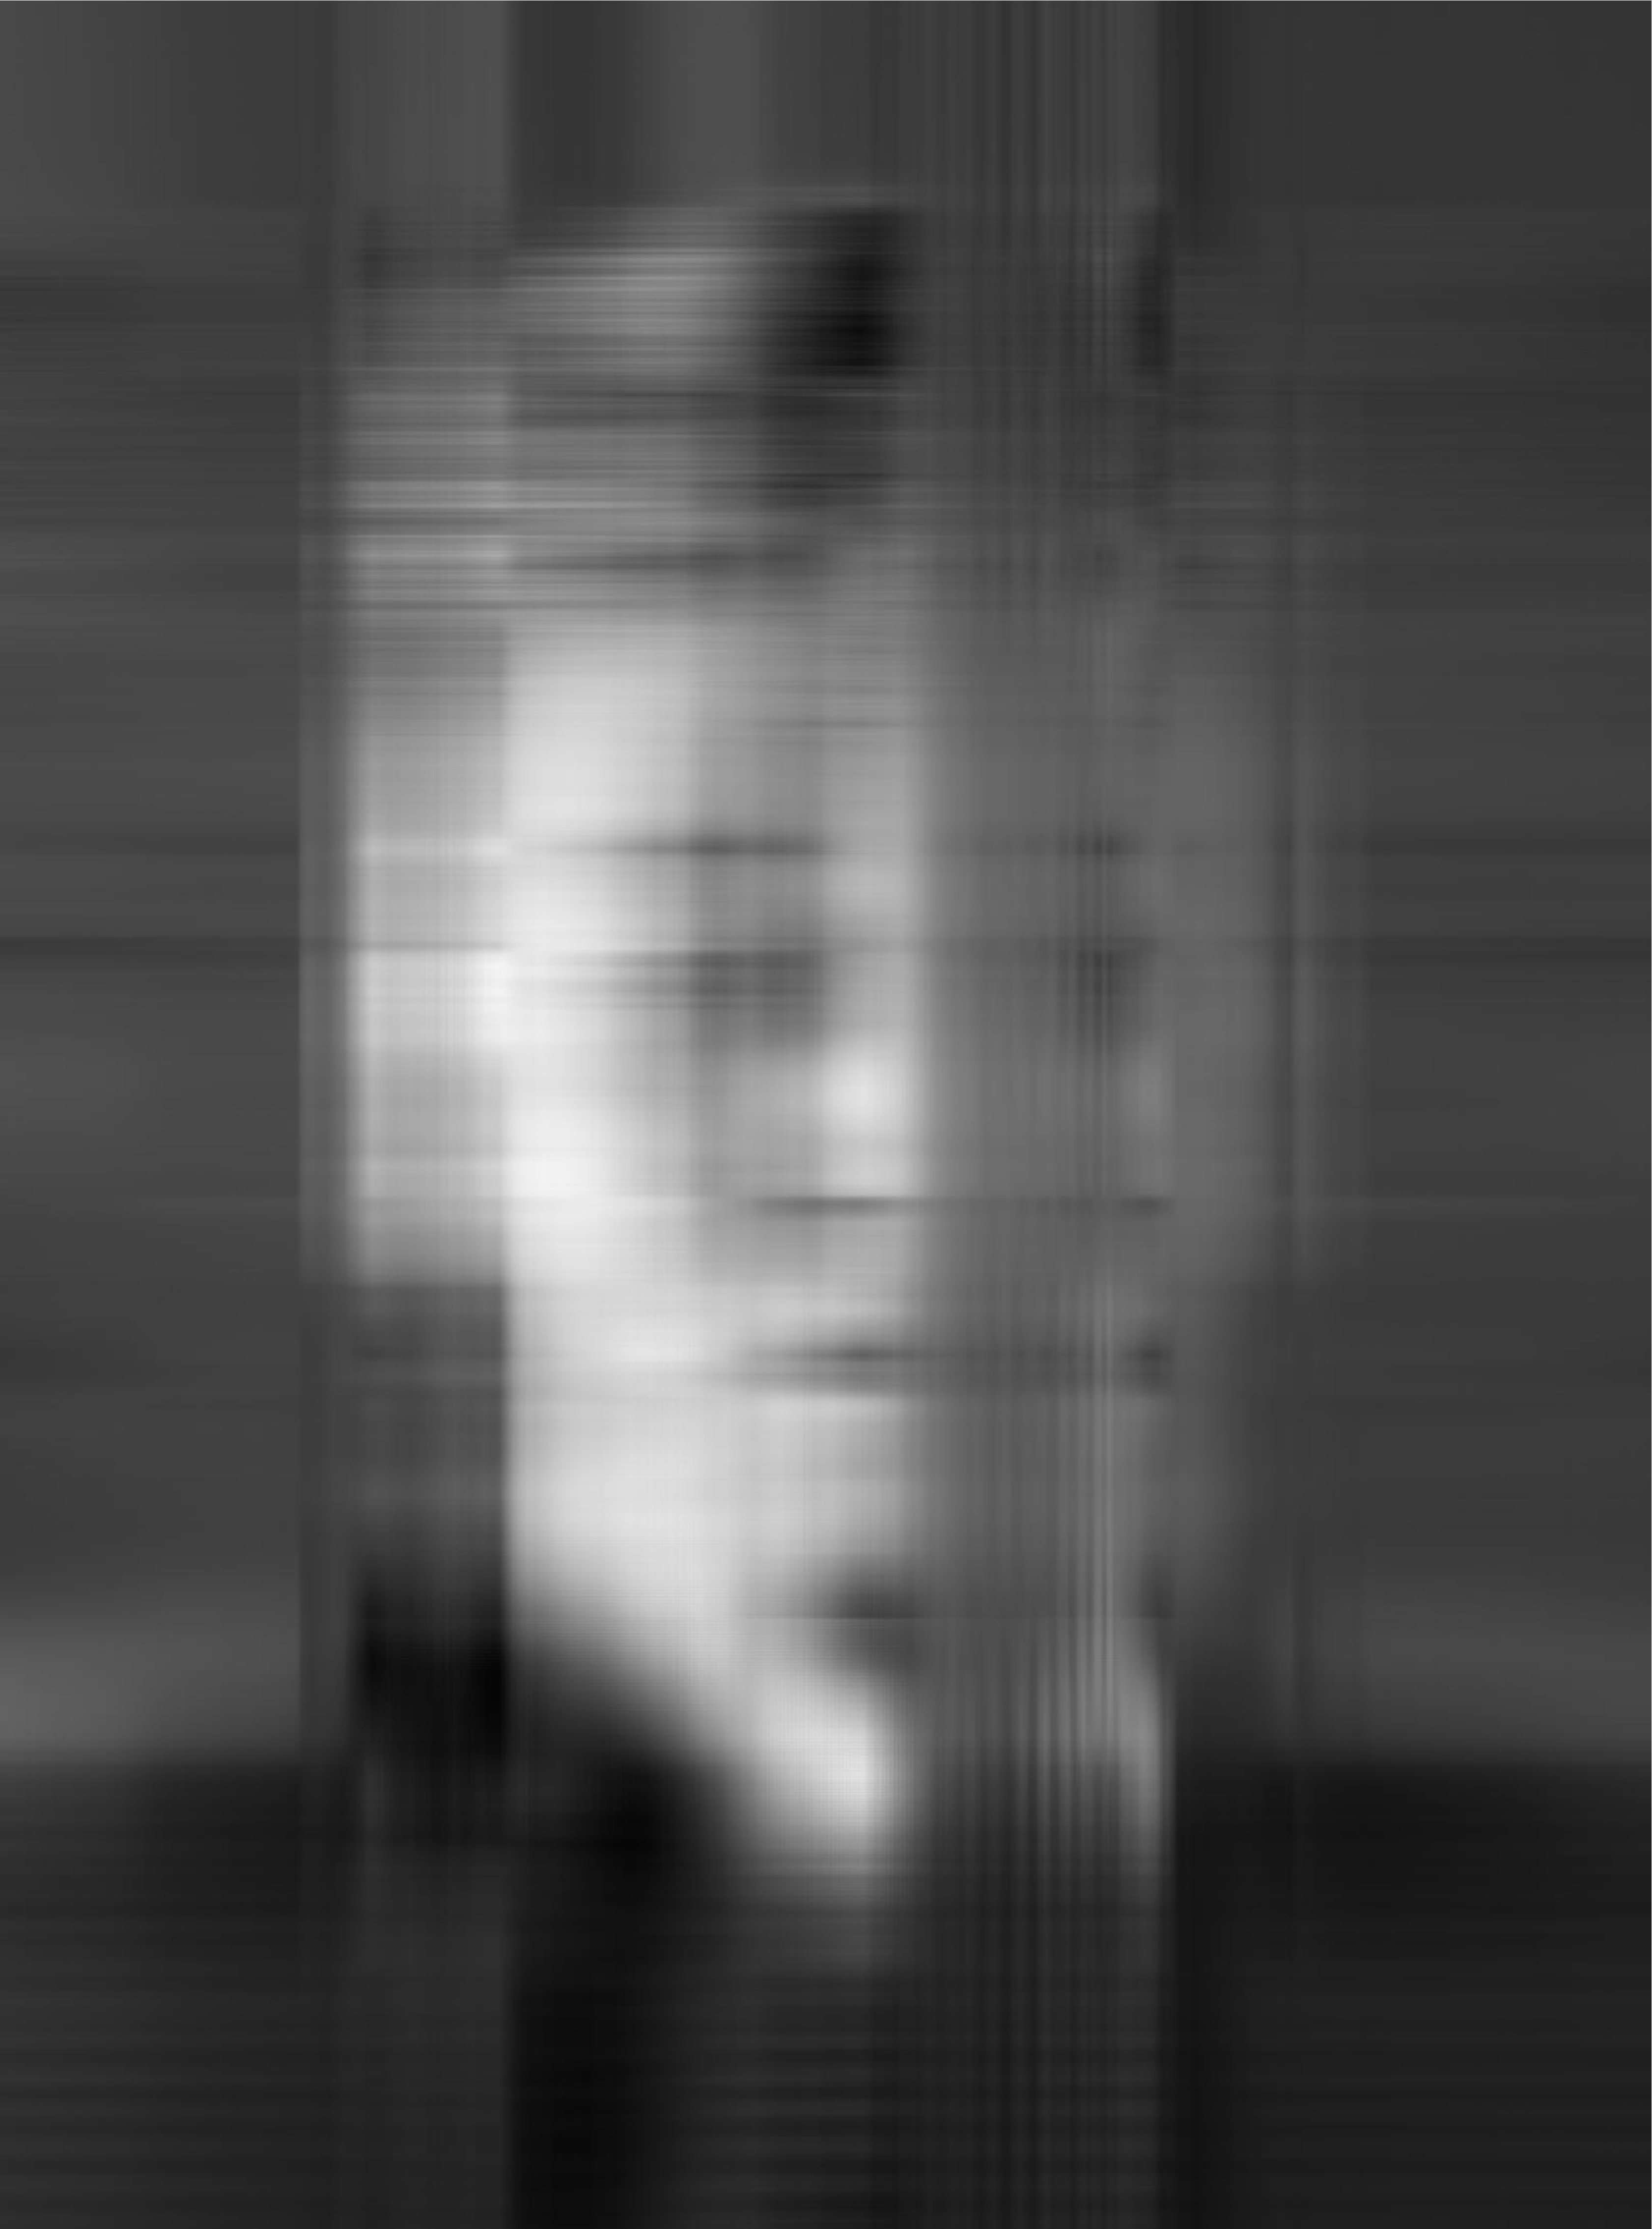
\includegraphics{image/gray_picture_r4.pdf}} \\
    \end{tabular}
  \end{itemize}
\end{frame}

\begin{frame}[t,fragile]{特異値分解による画像圧縮}
  \begin{itemize}
  \item 特異値の分布とランク$r$近似 ($1614 \times 2178$グレイスケール写真)
    
    \hspace*{-3em}\resizebox{0.27\textwidth}{!}{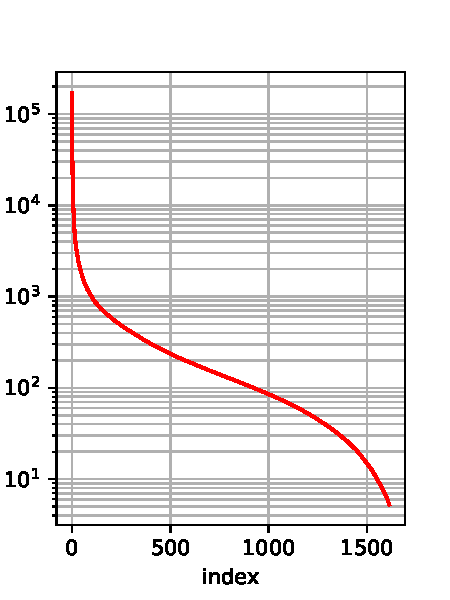
\includegraphics{image/singular_values.pdf}}

    \vspace*{-11em}\hfill
    \begin{tabular}{cccc}
      $r=1$ & $r=2$ & $r=3$ & $r=4$ \\
      \resizebox{0.15\textwidth}{!}{
\includegraphics{image/gray_picture_r1.pdf}} &
      \resizebox{0.15\textwidth}{!}{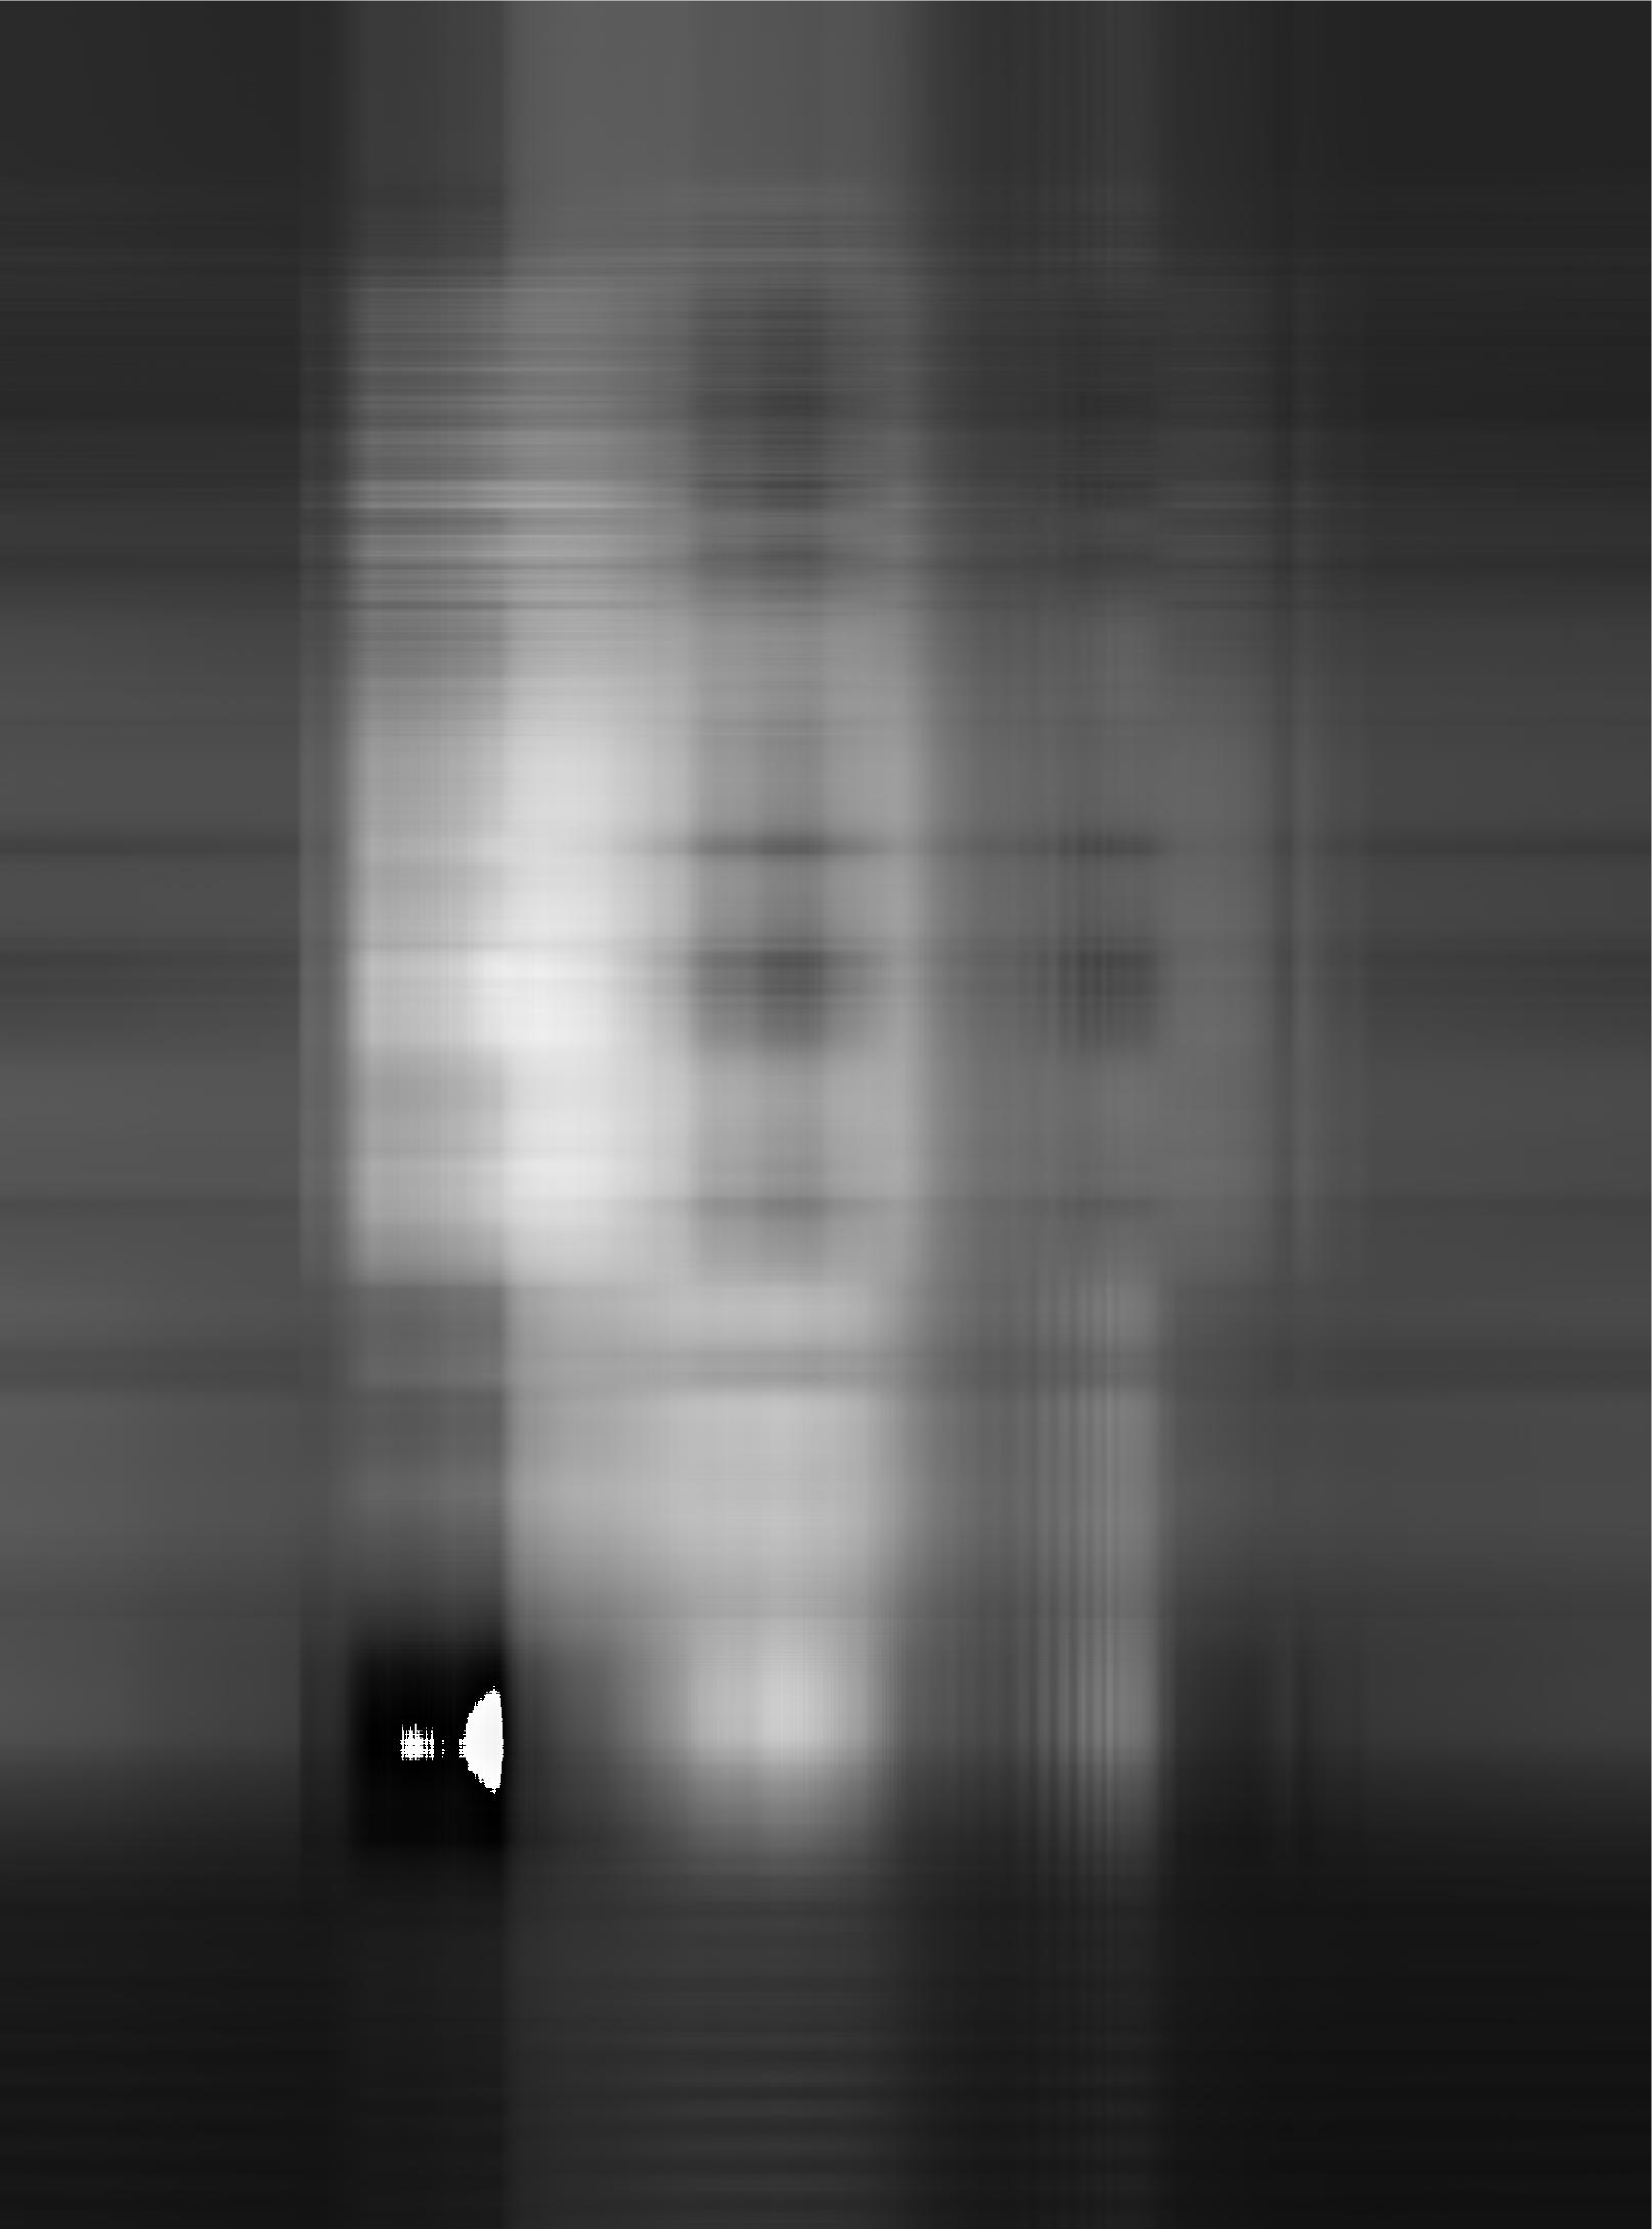
\includegraphics{image/gray_picture_r2.pdf}} &
      \resizebox{0.15\textwidth}{!}{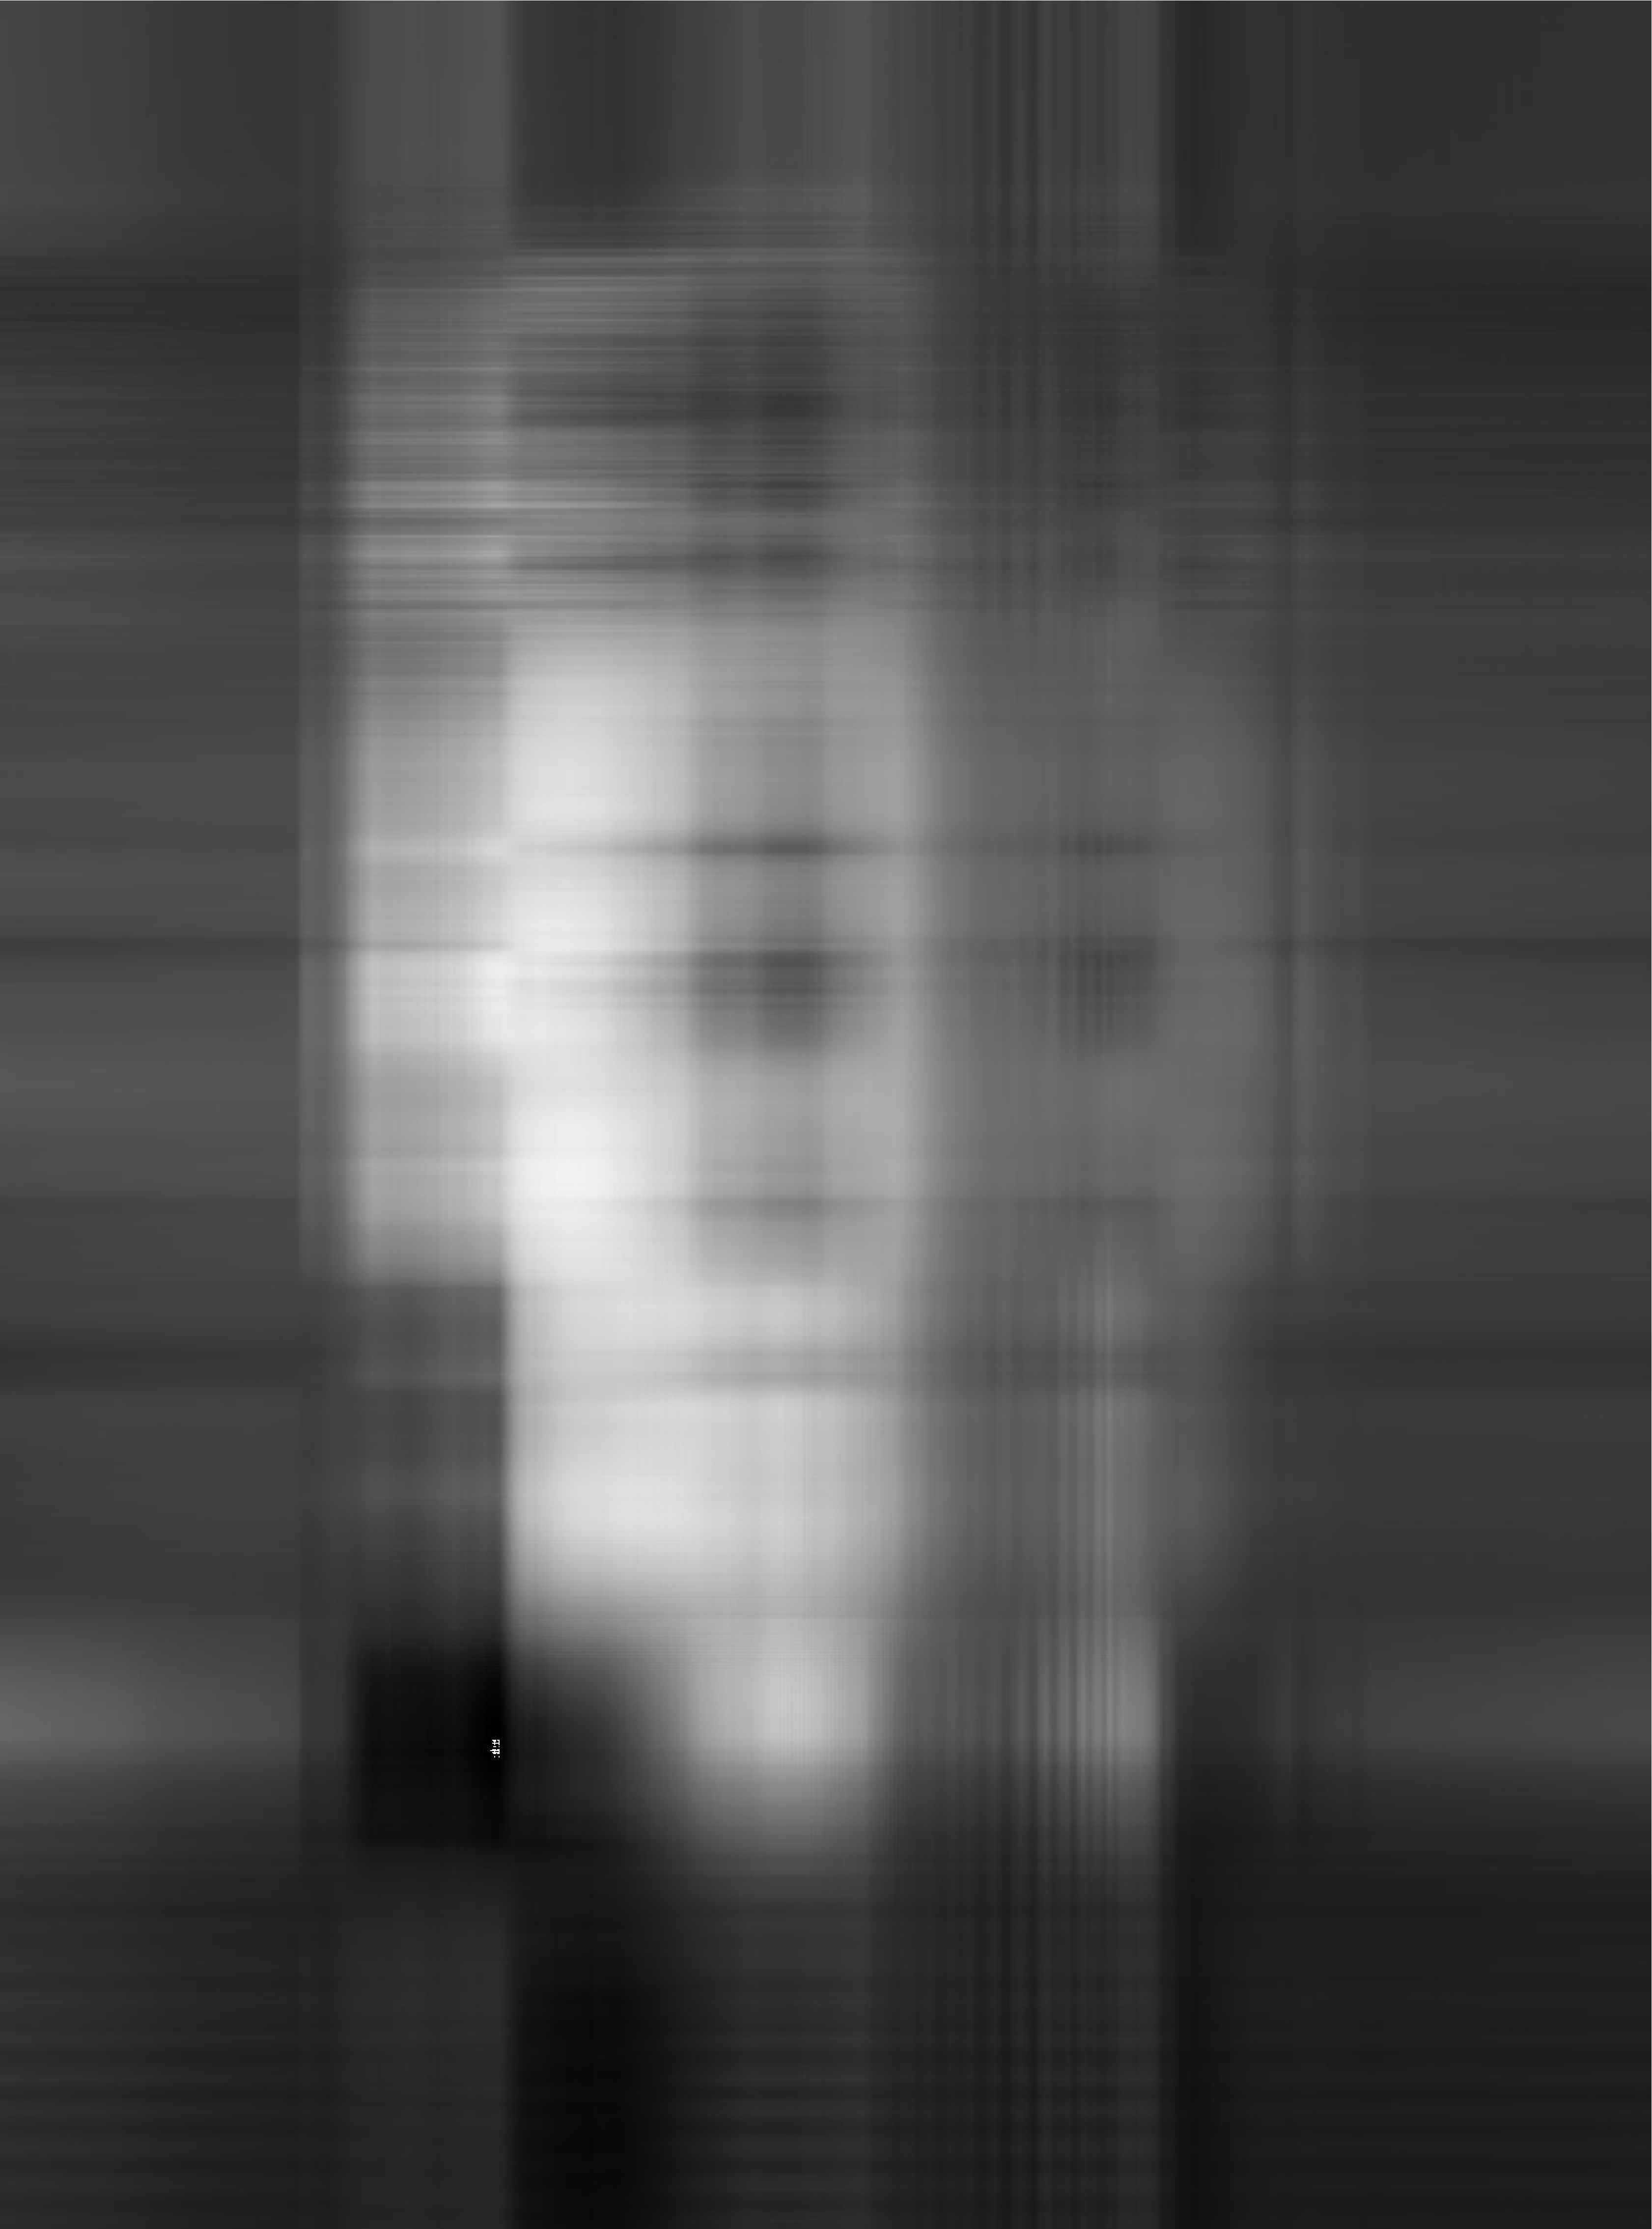
\includegraphics{image/gray_picture_r3.pdf}} &
      \resizebox{0.15\textwidth}{!}{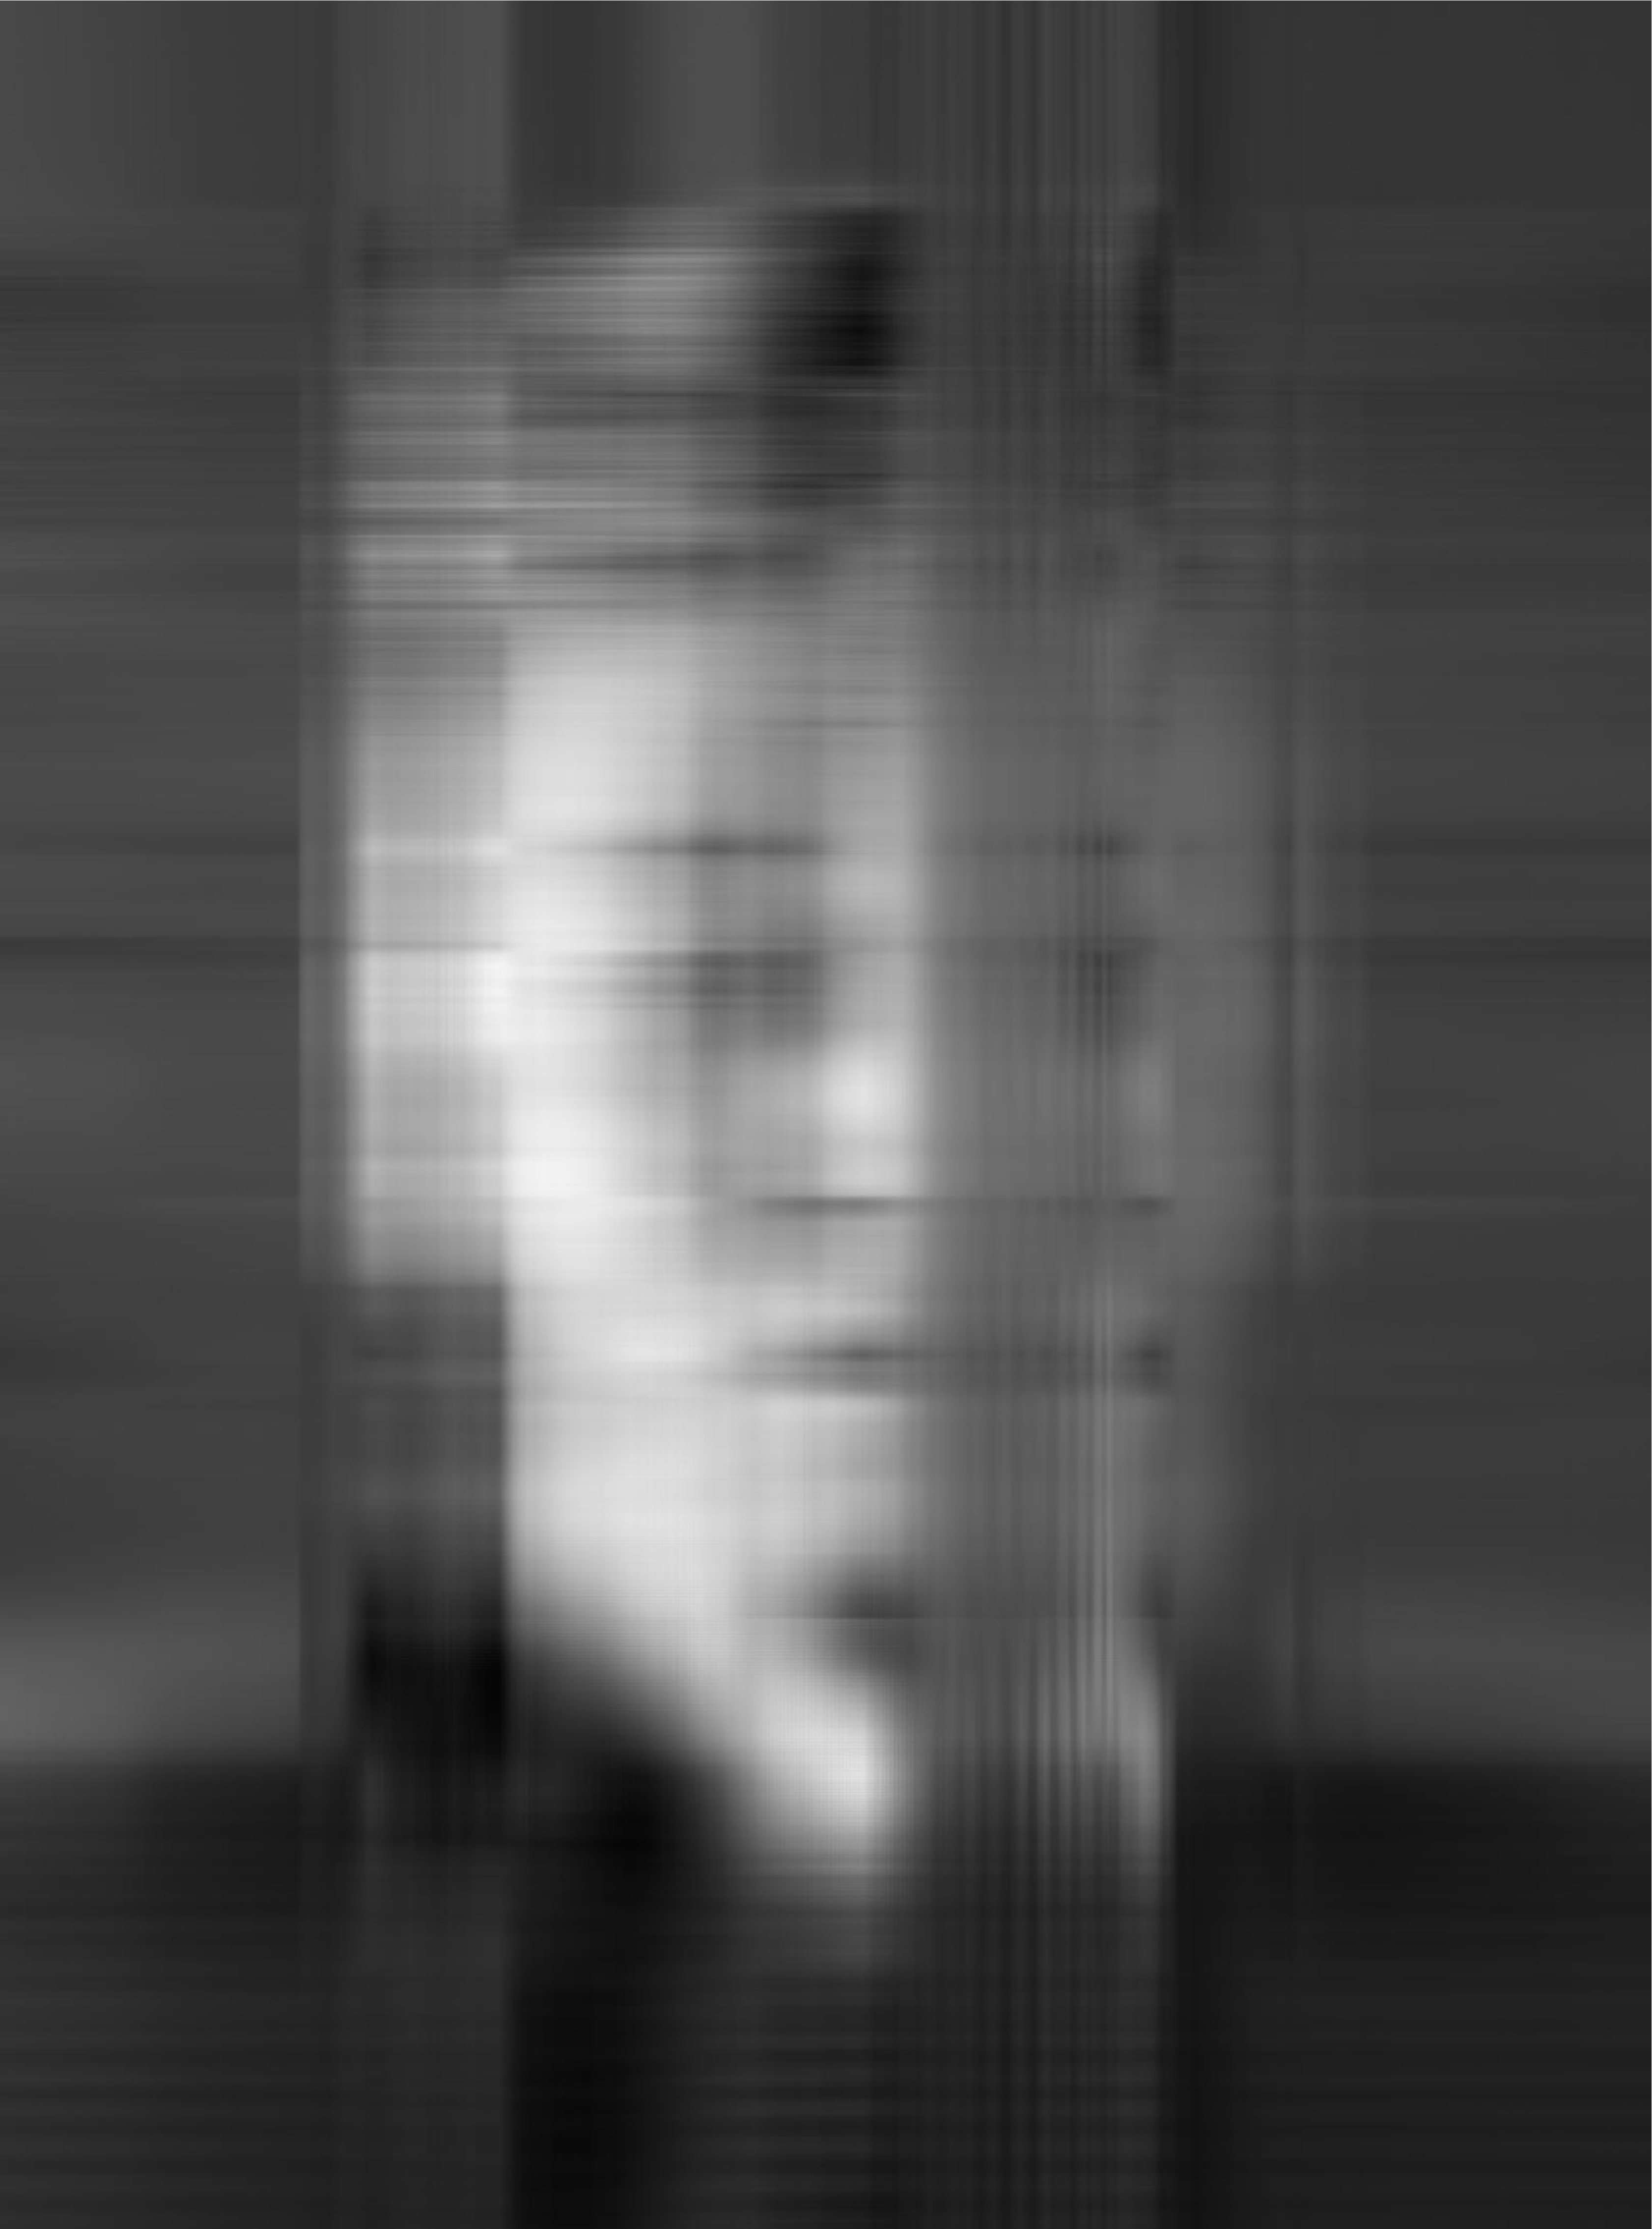
\includegraphics{image/gray_picture_r4.pdf}} \\
      $r=5$ & $r=10$ & $r=20$ & $r=50$ \\
      \resizebox{0.15\textwidth}{!}{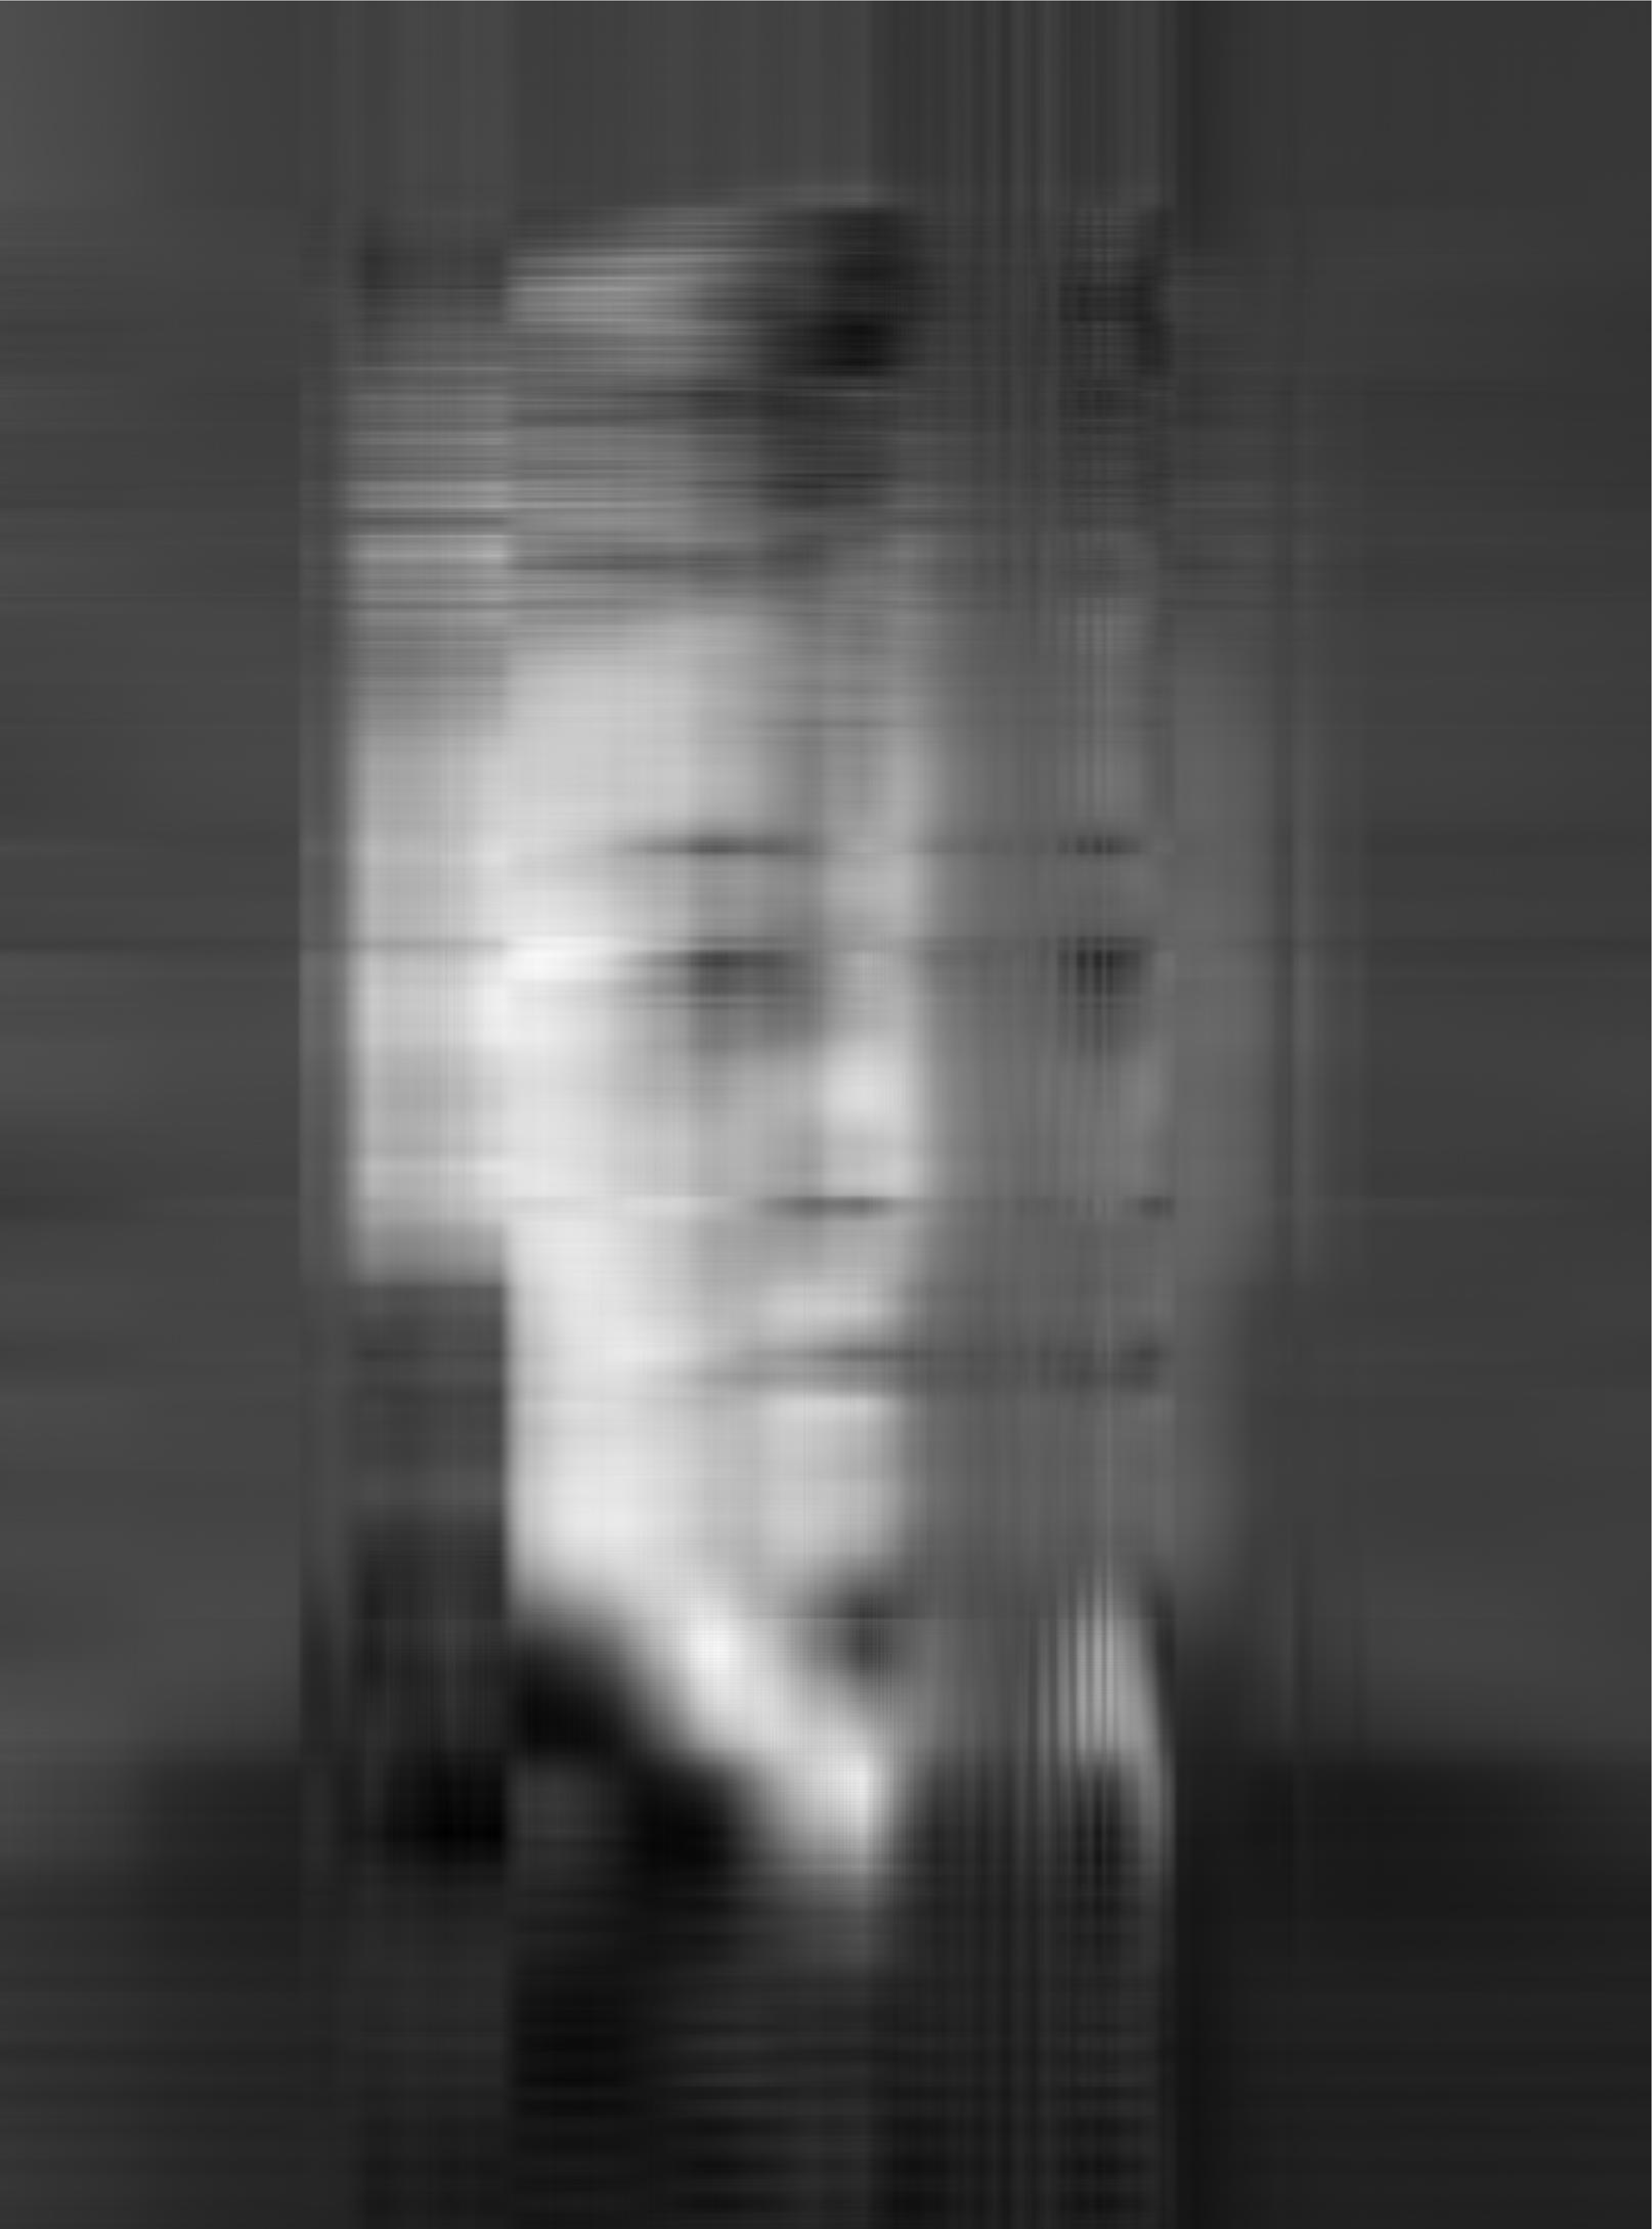
\includegraphics{image/gray_picture_r5.pdf}} &
      \resizebox{0.15\textwidth}{!}{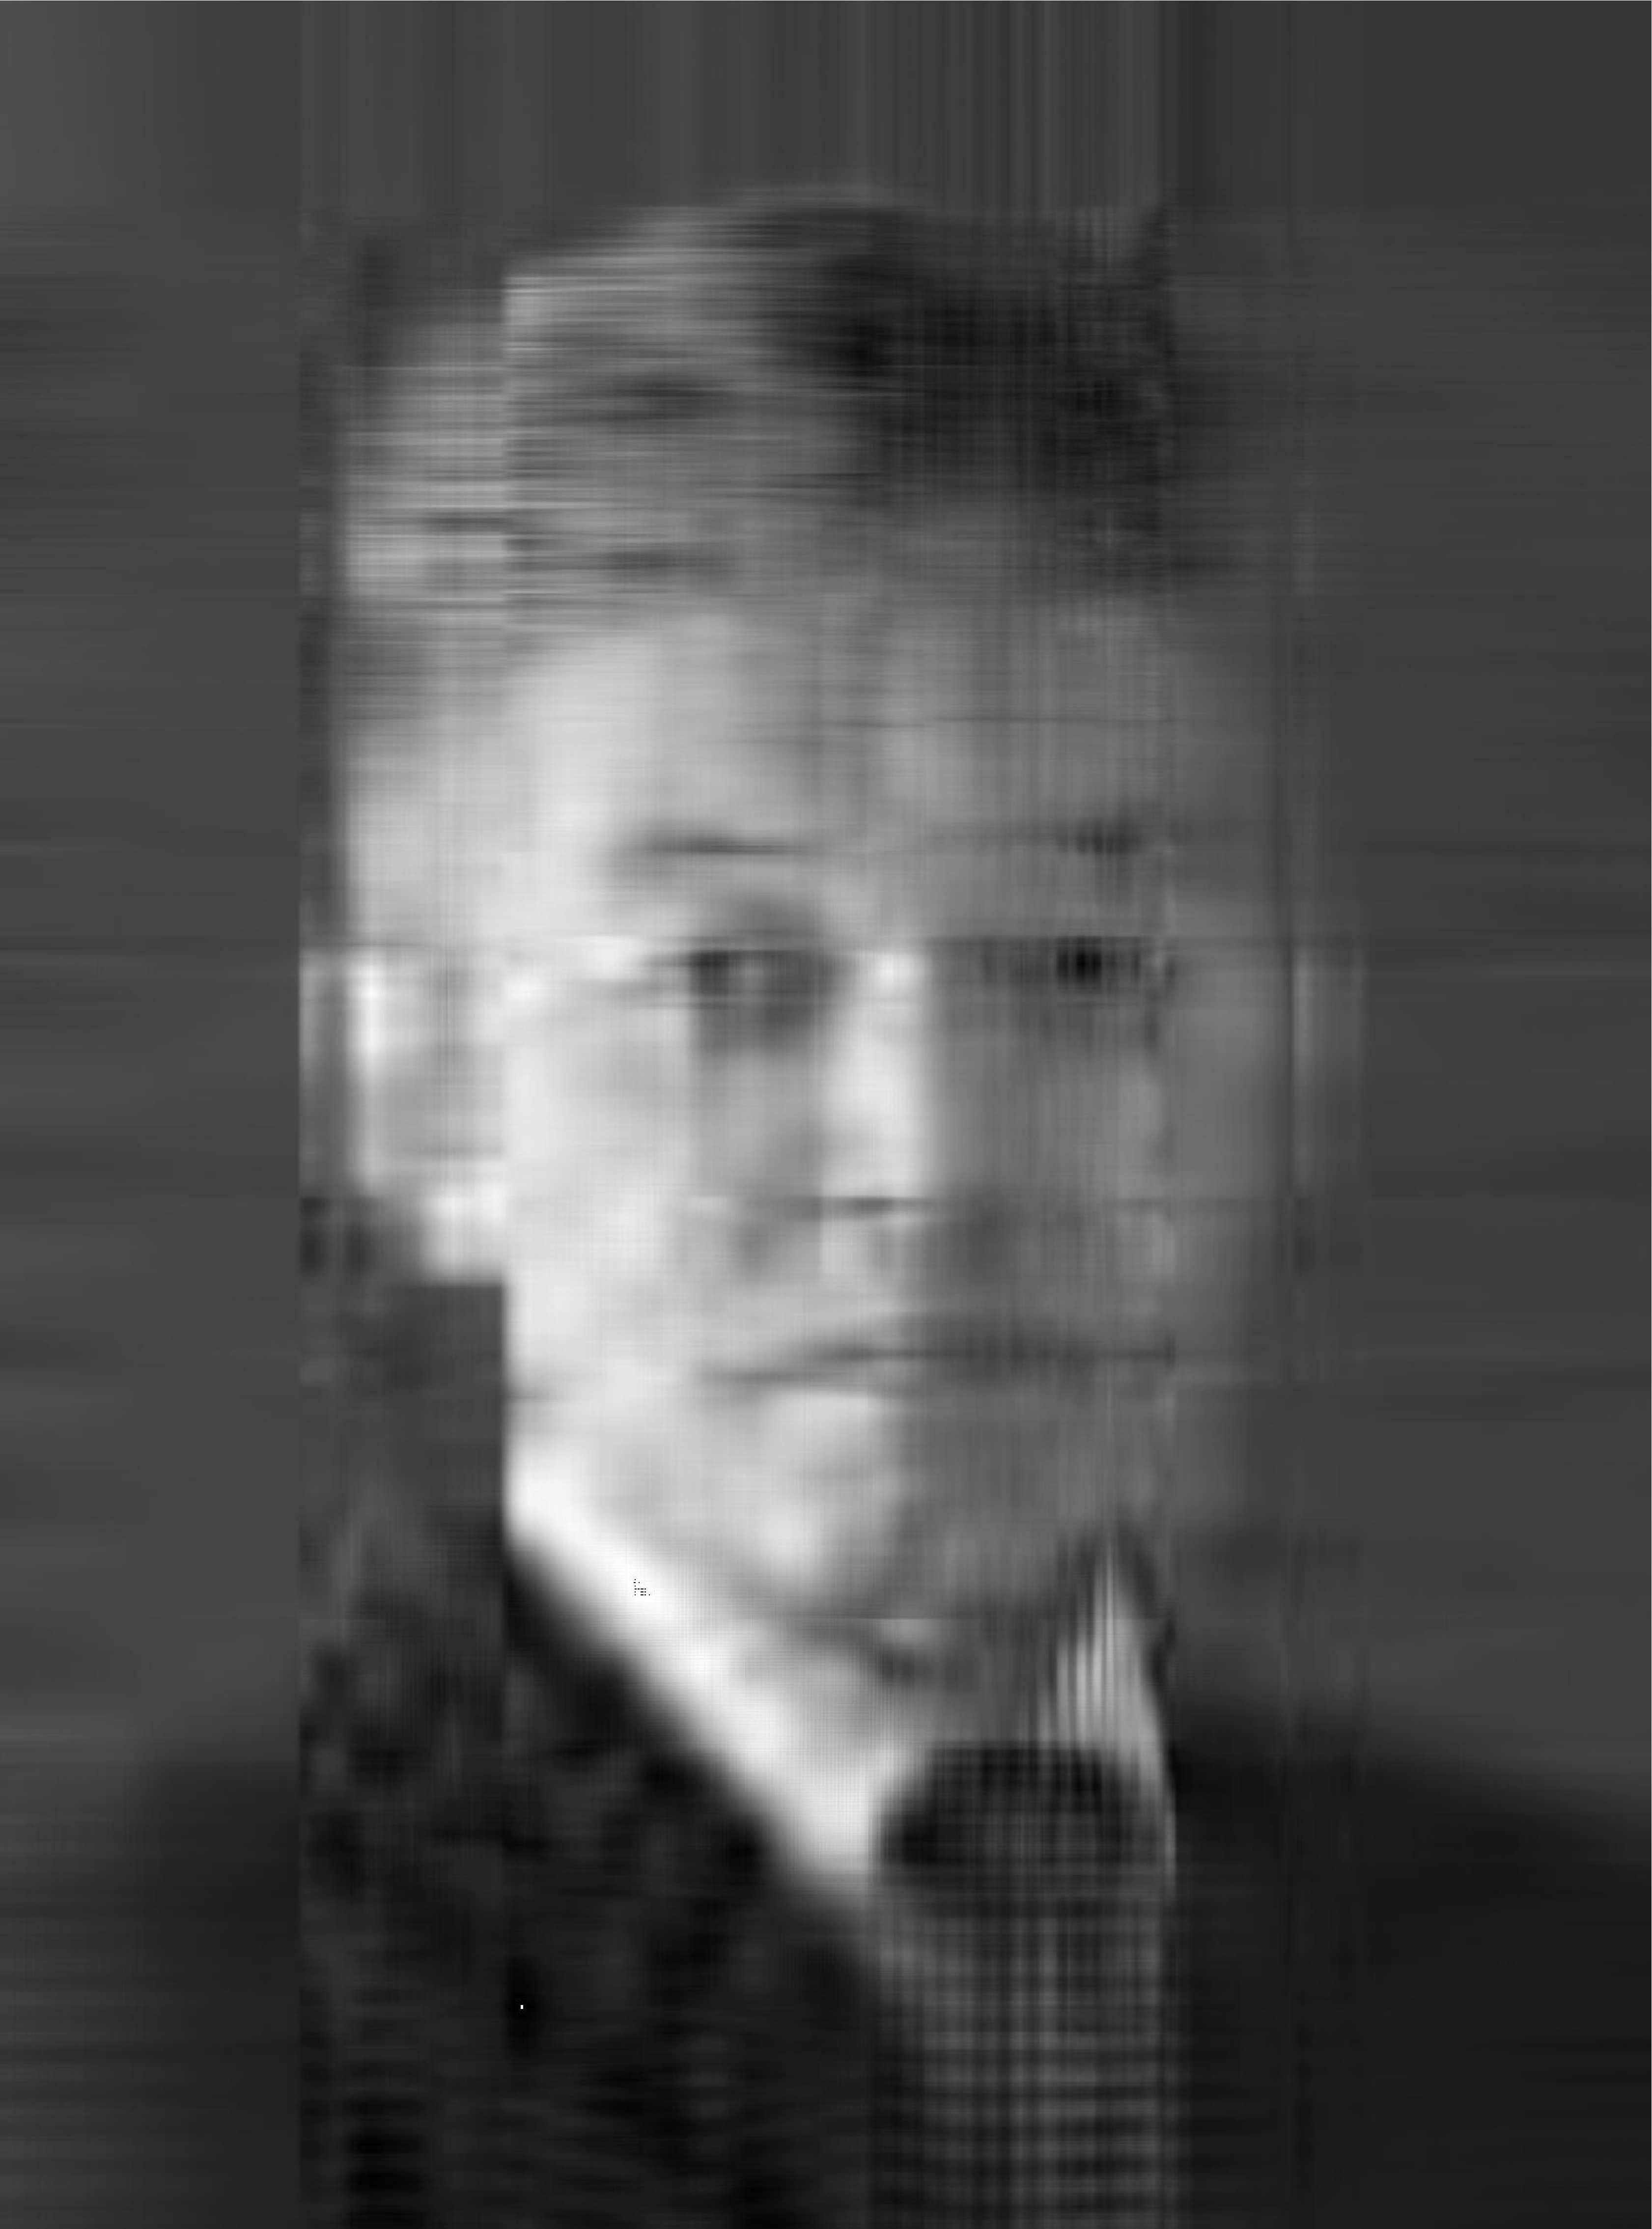
\includegraphics{image/gray_picture_r10.pdf}} &
      \resizebox{0.15\textwidth}{!}{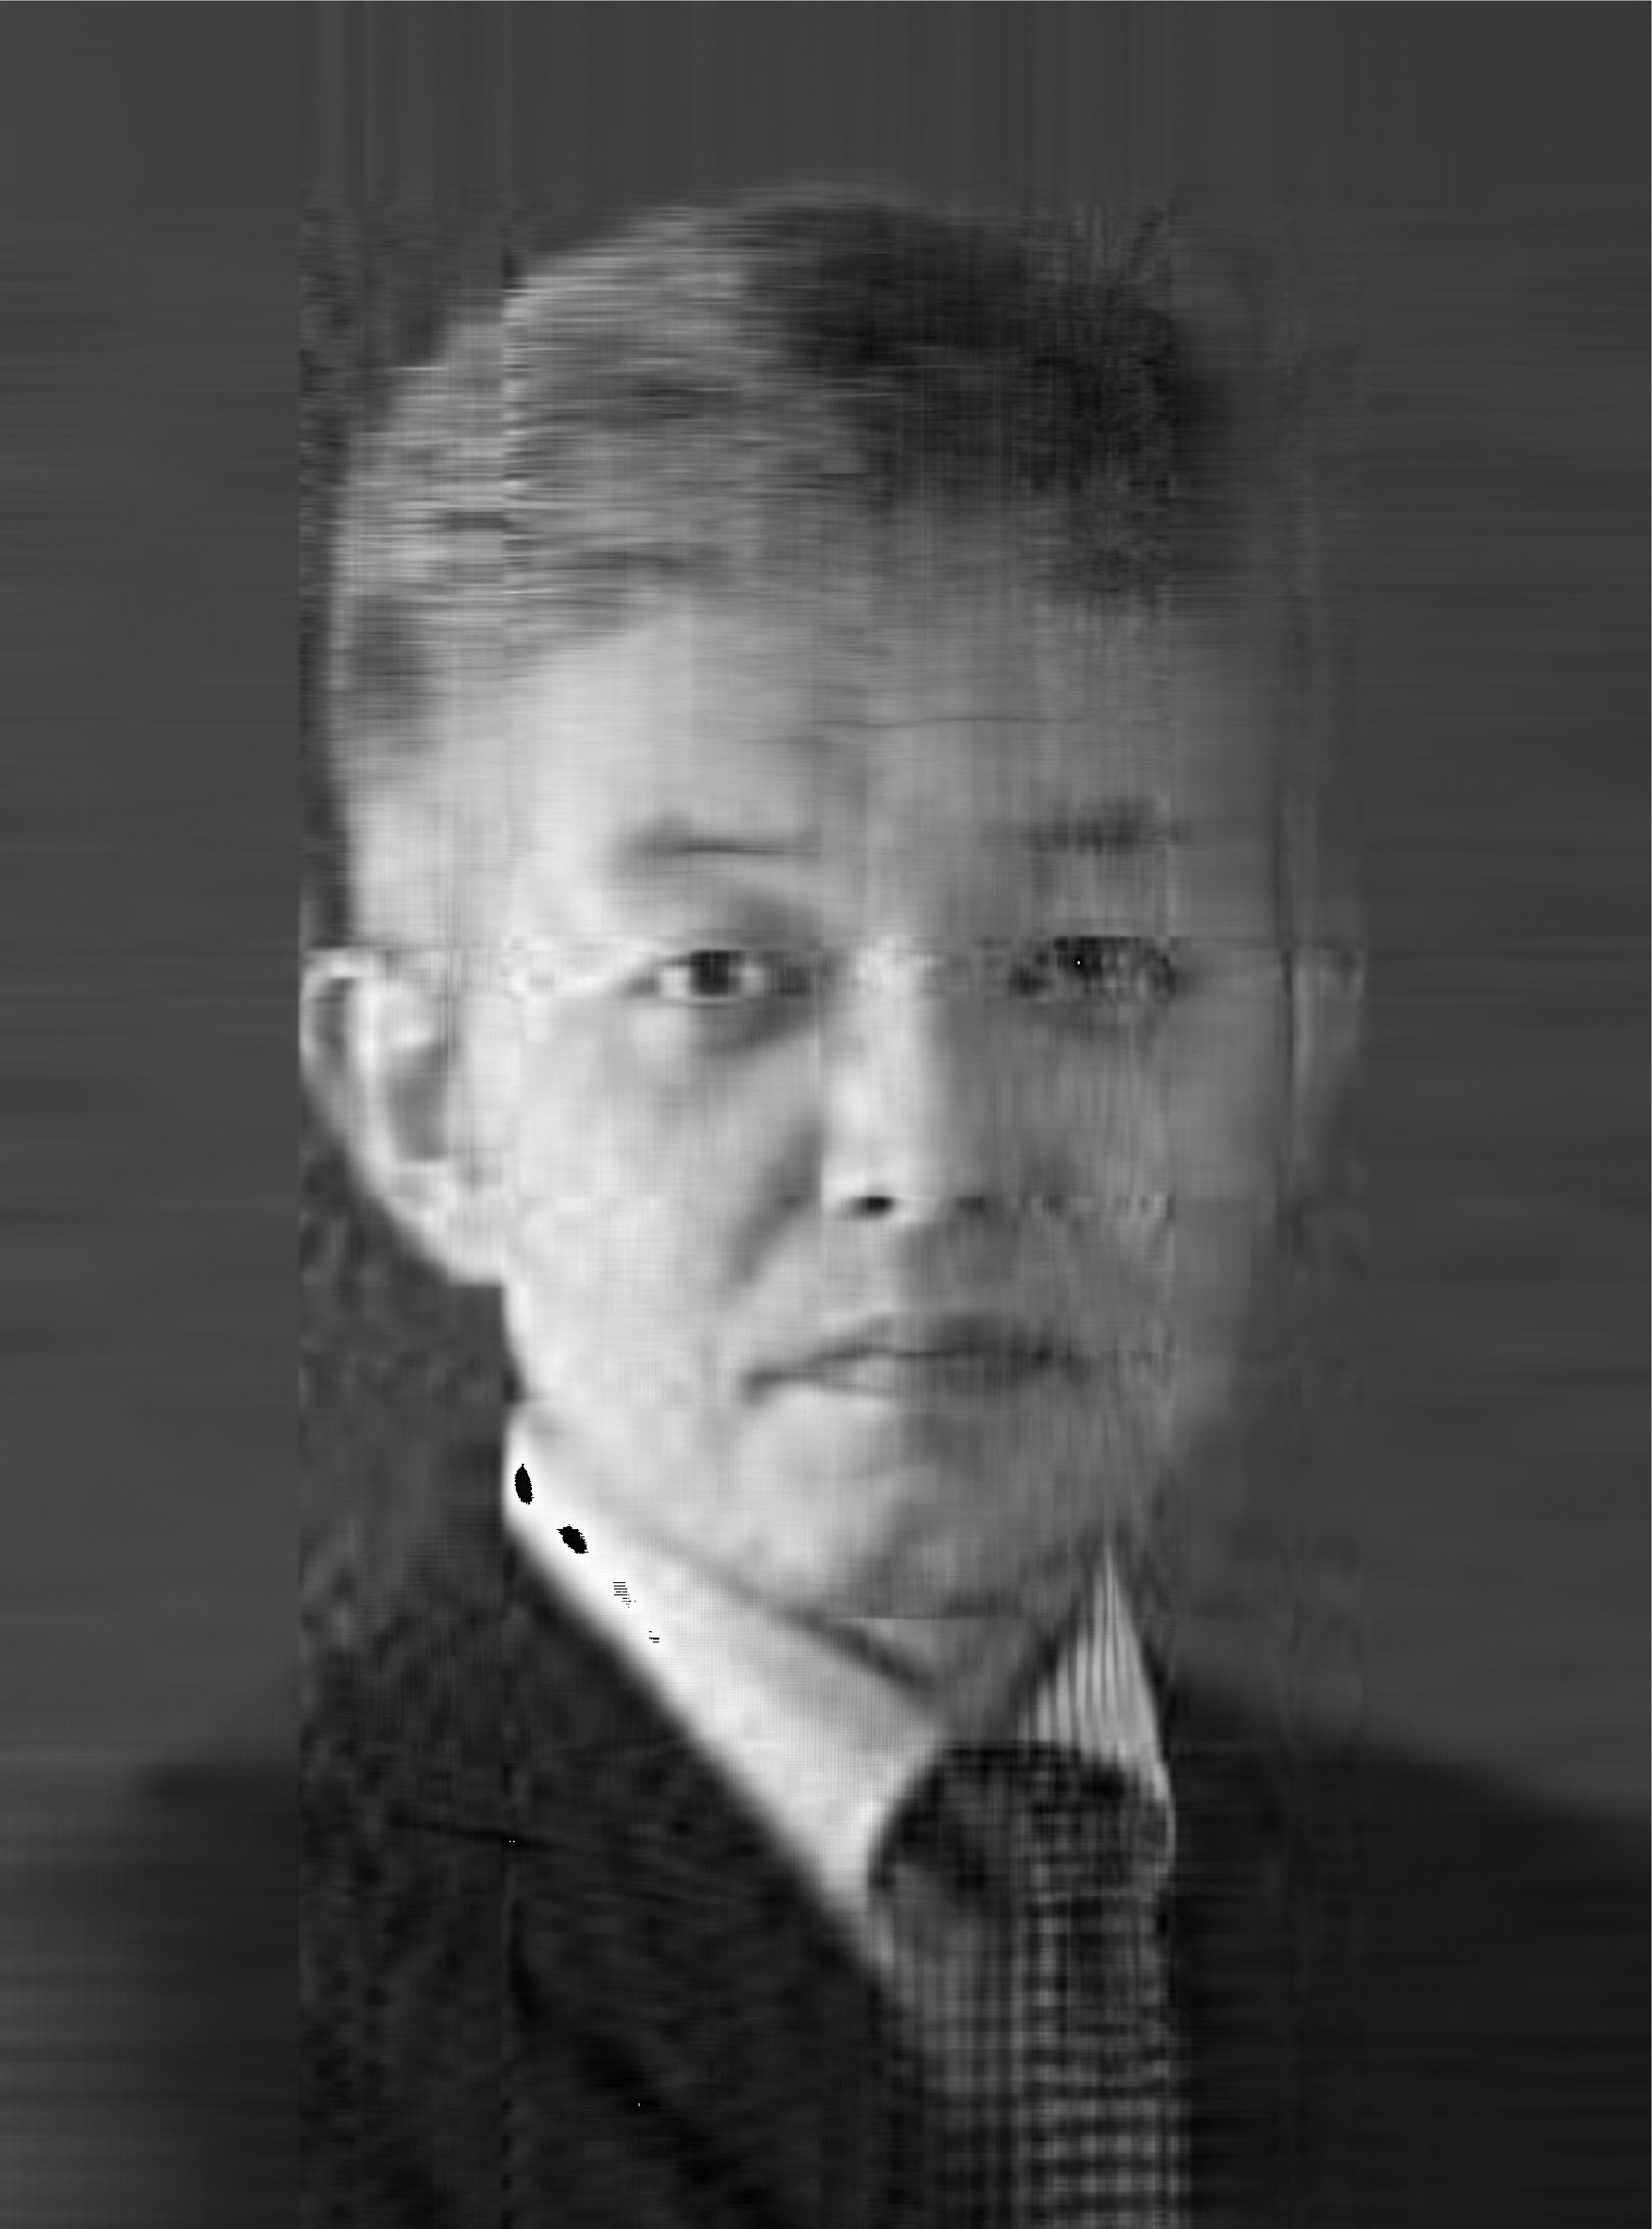
\includegraphics{image/gray_picture_r20.pdf}} &
      \resizebox{0.15\textwidth}{!}{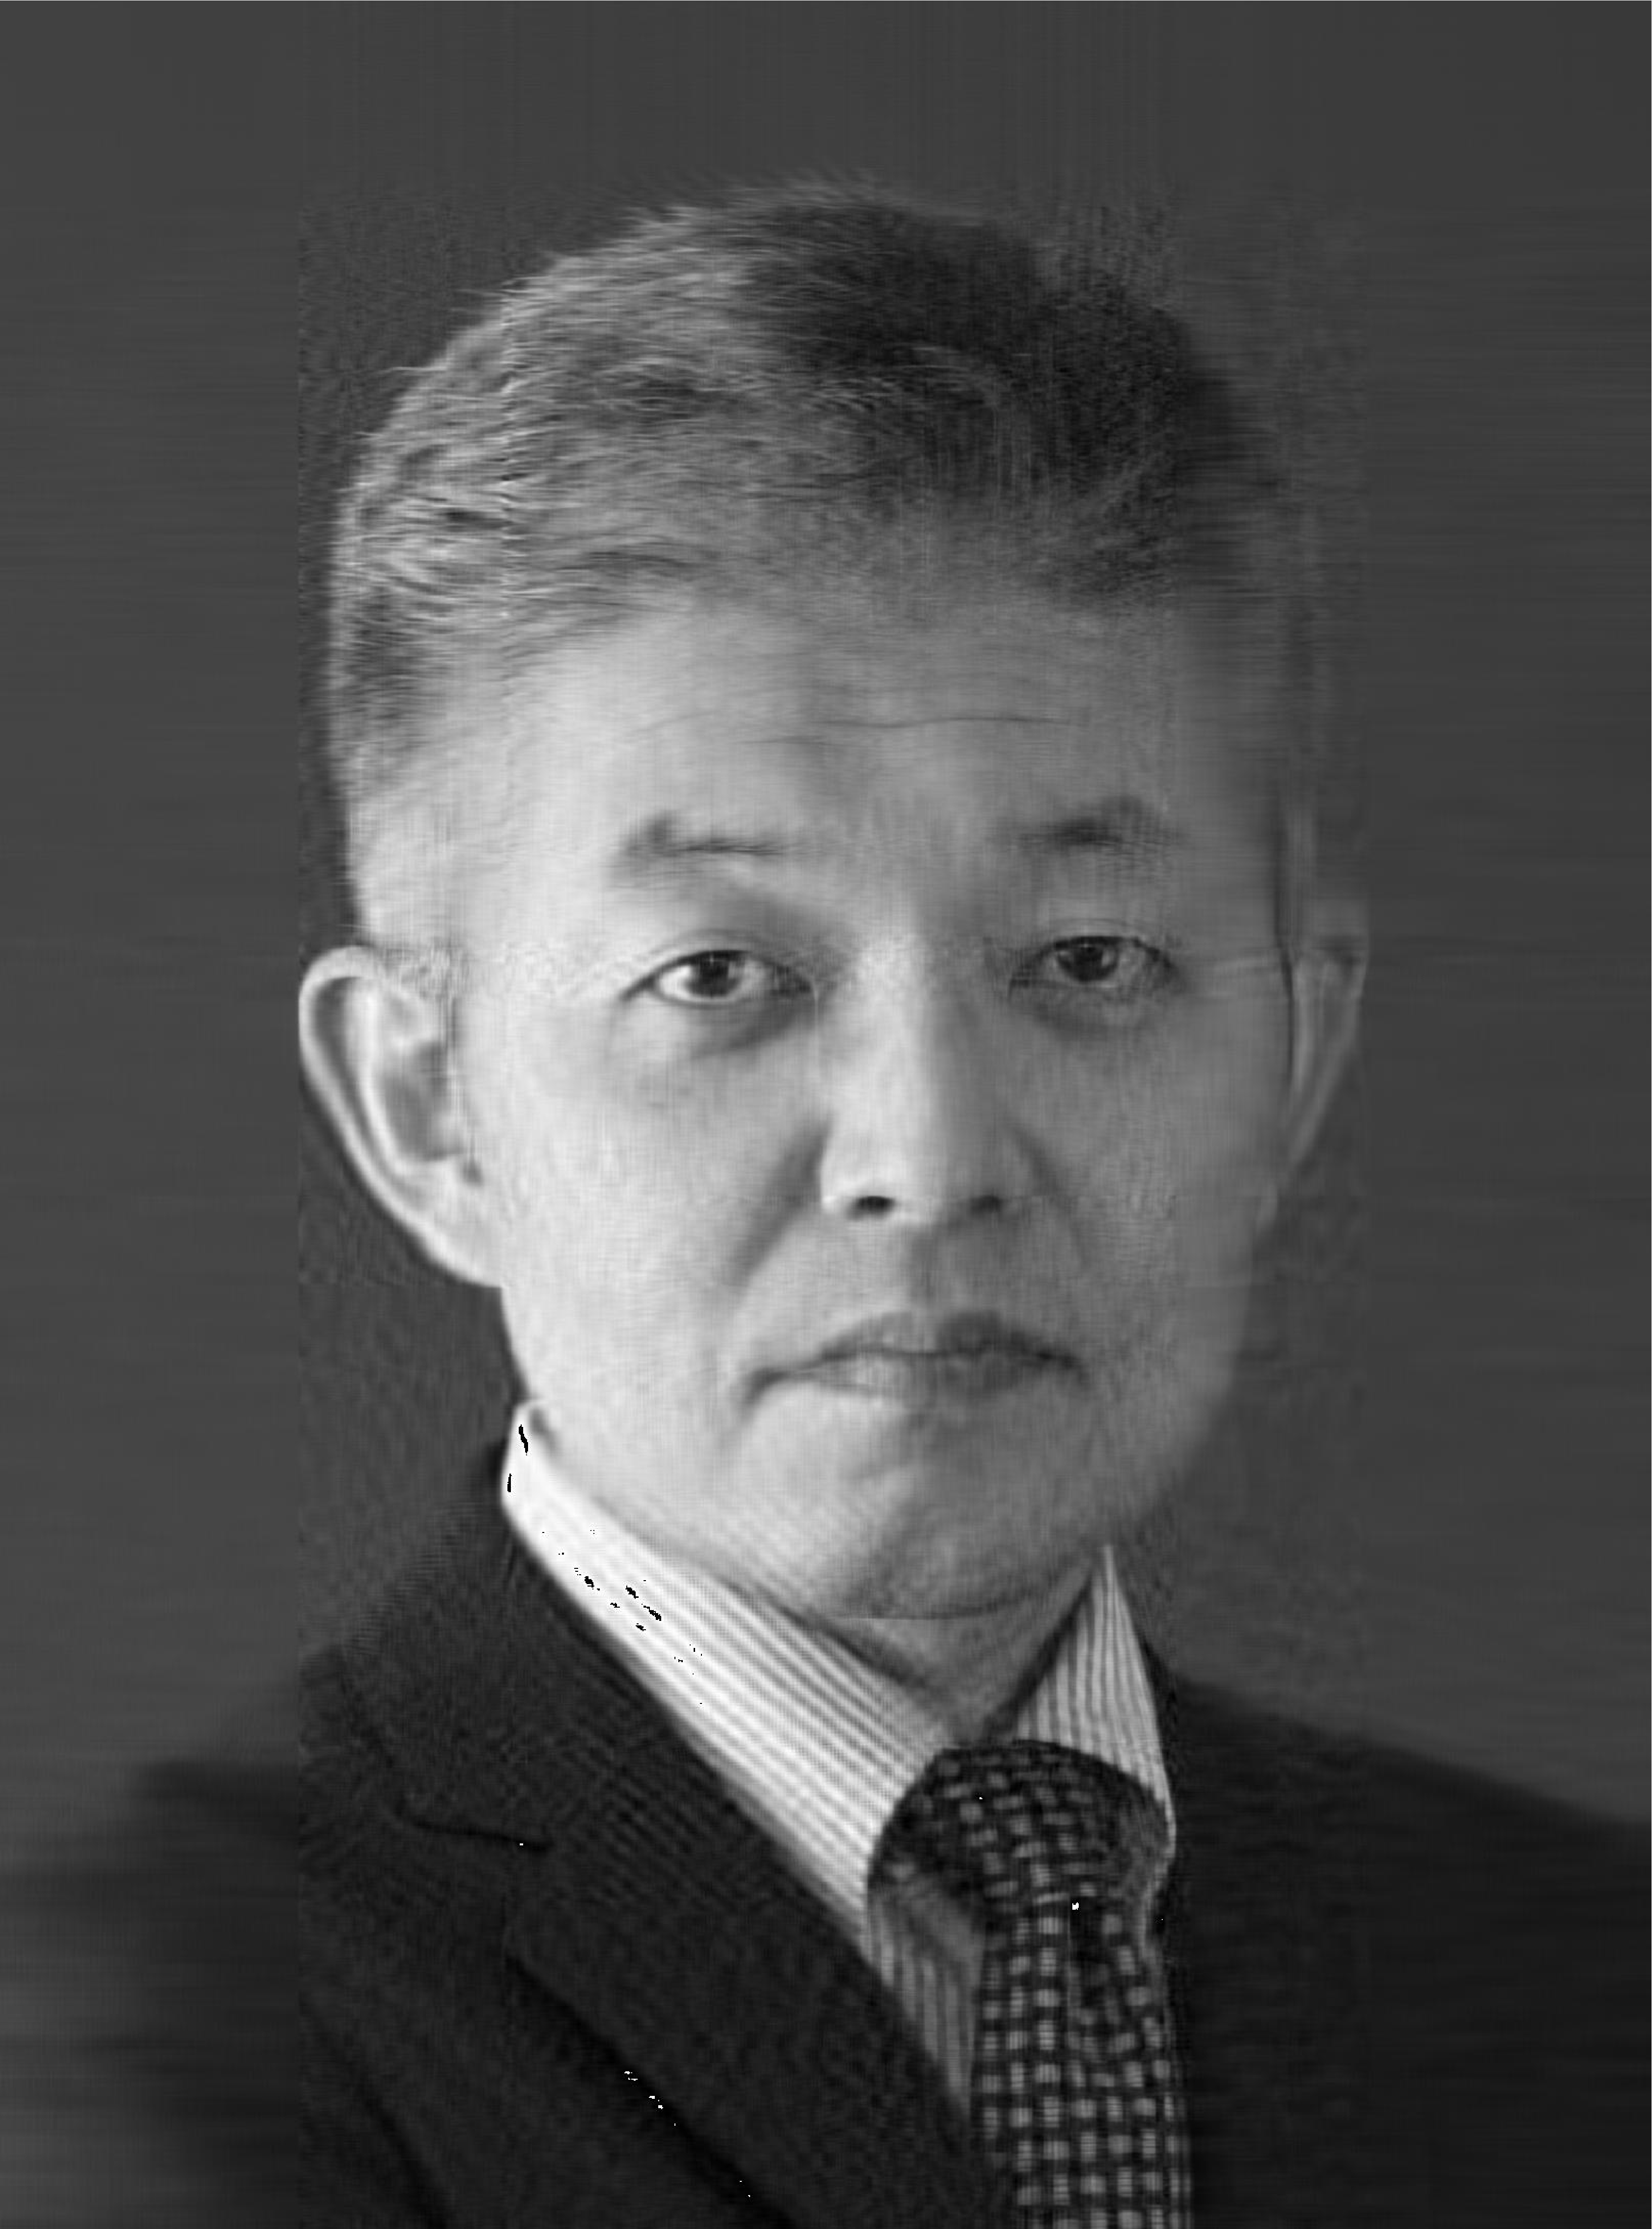
\includegraphics{image/gray_picture_r50.pdf}} \\
    \end{tabular}
  \end{itemize}
\end{frame}

\section{二重井戸ポテンシャル}

\begin{frame}[t,fragile]{二重井戸ポテンシャル中の粒子}
  \begin{itemize}
    %\setlength{\itemsep}{1em}
  \item 時間依存しないシュレディンガー方程式
    \begin{align*}
      \big[ -\frac{d^2}{dx^2} + V(x) \big] \psi(x) = E \psi(x)
    \end{align*}
    ($\hbar^2/2m = 1$となるように単位をとった)
  \item 二重井戸ポテンシャル
    \begin{align*}
      V(x) = \begin{cases}
        \infty & \text{$x < 0$, $x > 1$} \\
        0 & \text{$0 < x < a$, $b < x < 1$} \\
        v & \text{$a < x < b$}
      \end{cases}
    \end{align*}
    ただし、$0<a<b<1$とする
  \item 境界条件: $\psi(0) = \psi(1) = 0$、$0 < x < 1$で$\psi(x)$とその導関数が連続
  \end{itemize}
\end{frame}

\begin{frame}[t,fragile]{シュレディンガー方程式の解法}
  \begin{itemize}
    % \setlength{\itemsep}{1em}
  \item シューティング
    \begin{itemize}
    \item 計算機実験I (L2)
    \item シューティングに用いる積分法: 2階常微分方程式の2次元1階連立微分方程式への書き換え、オイラー法とその改良、Numerov法
    \end{itemize}
  \item ハミルトニアンの対角化
    \begin{itemize}
    \item 計算機実験I (L4)
    \item 対角化手法: ハウスホルダー法(LAPACK)、べき乗法、Lanczos法
    \end{itemize}
  \item 変分法: 変分関数のパラメータの最適化
  \item その他の方法: 手で解けるところはあらかじめ解いて次元を減らす
  \item それぞれのコスト(=計算時間・メモリ)は?
  \end{itemize}
\end{frame}

\section{実習その3}

\begin{frame}[t,fragile]{EX3-1: サンプルプログラムの実行}
  \begin{itemize}
    %\setlength{\itemsep}{1em}
  \item[3-1-1] ガウスの消去法のサンプルプログラム(\href{https://github.com/todo-group/computer-experiments/blob/master/exercise/linear_system/gauss.c}{exercise/linear\_system/gauss.c})をコンパイル・実行せよ。実行時にコマンドライン引数に行列の内容が書かれたファイル名({\tt input1.dat})を指定する必要があることに注意
\begin{lstlisting}
$ cc gauss.c -o gauss
$ ./gauss input1.dat
\end{lstlisting}
  \item[3-1-2] LU分解のサンプルプログラム(\href{https://github.com/todo-group/computer-experiments/blob/master/exercise/linear_system/lu_decomp.c}{exercise/linear\_system/lu\_decomp.c})をコンパイル・実行せよ。コンパイル時にLAPACKをリンク({\tt -llapack})する必要があることに注意(ハンドブック3.1.6節)
\begin{lstlisting}
$ cc lu_decomp.c -o lu_decomp -llapack
$ ./lu_decomp input1.dat
\end{lstlisting}
  \end{itemize}
\end{frame}

\begin{frame}[t,fragile]{EX3-2: ピボット選択、境界条件}
  \begin{itemize}
    %\setlength{\itemsep}{1em}
  \item[3-2-1] {\tt gauss.c}では、ピボット選択を行っていないため、入力が{\tt input2.dat}の場合には正しい解が得られない。ピボット選択を行うよう{\tt gauss.c}を修正せよ
  \item[3-2-2] \href{https://github.com/todo-group/computer-experiments/blob/master/exercise/linear_system/laplace_lu.c}{exercise/linear\_system/laplace\_lu.c}では、ディリクレ型の境界条件[$u(0,y) = \sin(\pi y)$, $u(x,0)=u(x,1)=u(1,y)=0$]のもとでのラプラス方程式の解をLU分解により求めている。境界条件を変えてみて解がどのように変化するか、Gnuplotを用いてプロットして確認せよ(Gnuplotの{\tt splot}コマンドを使う)
  \end{itemize}
\end{frame}

\begin{frame}[t,fragile]{EX3-3: ヤコビ法、ガウス・ザイデル法、SOR法}
  \begin{itemize}
    %\setlength{\itemsep}{1em}
  \item[3-3-1] \href{https://github.com/todo-group/computer-experiments/exercise/blob/master/linear_system/laplace_jacobi.c}{exercise/linear\_system/laplace\_jacobi.c}は、作りかけのヤコビ法のプログラムである。収束判定のコードを追加し、プログラムを完成せよ。計算結果や計算速度を{\tt laplace\_lu.c}と比較せよ
  \item[3-3-2] ヤコビ法のプログラム({\tt lapalace\_jacobi.c})を元に、ガウス・ザイデル法、SOR法のプログラムを作成せよ。収束までの回数を比較せよ。
特にSOR法の場合、パラメータ$\omega$の選び方により、どのように収束回数が変化するか観察し、最適な$\omega$の値について考察せよ
  \end{itemize}
\end{frame}


\end{document}
